\chapter{Diffusion Models for Surrogate Simulation}

An incredible amount of computing resources is required to keep up with the demands for simulated events at the LHC experiments.
Accurate Monte Carlo (MC) simulations are crucial, as they serve as the foundation for hypothesis tests that compare physics models with collision data.
There is growing interest in utilizing fast surrogate models for event and detector simulations.
Deep generative models have shown great success in the wider field of machine learning, most notably for image generation, and have reached a point where they are showing promise in improving the fidelity and speed of fast simulation approaches.
In addition to fast simulation, accurate generative models on collider data can also be used for template-based anomaly detection or the inverse problem of unfolding.

One of the early objectives of this thesis was to develop a generative model specifically for collider data, which proved uniquely challenging.
Unlike the data used in computer vision, it is inherently point-like, and unlike the data used in language modelling, it is unordered and continuous.
These characteristics make physics data well suited to graphical representations, hence the success of graph networks in jet tagging, as discussed in \Cref{ch:spice}.
Set generation methods, typically benchmarked on the ShapeNet dataset~\cite{ShapeNet}, provided a natural starting point for this work.

Initial efforts began with developing a graph-based VAE~\cite{SetVAE}, using a graph network decoder to transform pure noise into a reconstructed point cloud conditioned on the latent space.
While this approach worked on ShapeNet, it failed to generate high-quality samples of particle physics data.
The primary issue was identifying a suitable permutation-invariant loss term for the set reconstruction.
Various attempts were made, including modifications to Sinkhorn~\cite{Sinkhorn}, Chamfer, and optimal transport losses, as well as physically motivated metrics specific to collider data~\cite{MetricSpaceCollider}, all yielding suboptimal results.

Other research groups explored graph networks trained as GANs~\cite{MPGAN, EPICGAN}, achieving some success while encountering the typical drawbacks of GANs, detailed in \Cref{ch:generative_models}.

During this time, diffusion models started to gain prominence.
The diffusion generation task is similar to what was attempted with the VAE.
However, as the training objective is denoising rather than full generation, it is already permutation equivariant.
Therefore, it could be achieved using any standard loss function.

This chapter summarizes a collection of work to develop models for the conditional generation of set data, including particle physics jets~\cite{PCJedi, EpicJedi, PCDroid} and full events~\cite{PIPPIN}.
It also covers the use of these models for template-based anomaly detection~\cite{Drapes, RadOT}.

\section{\pcjedi}

A practical initial task for developing a generative model for collider data is generating individual particle physics jets.
These collimated showers of hadrons produce electrically charged and neutral particles within a cone originating from the interaction point.
Jet formation involves transitioning from colour-charged partons, explainable via perturbative QCD, to a collection of colour-singlet hadrons, leptons, and photons interacting with the detector material.
While both regimes are well understood, the transition between them is not and continues to be a focal point of ongoing research.

Parton showers are iteratively constructed using a Markovian algorithm that stochastically transitions an $n$-parton state to an $(n+1)$-parton state.
Eventually, these states are mapped to a collection of colour-singlet hadrons in a process called hadronization.
The showering and hadronization processes require dedicated tools such as \pythia~\cite{Pythia8}, \sherpa~\cite{Sherpa}, and \herwig~\cite{Herwig}.
The final set of hadrons, along with any leptons or photons, are referred to as the jet constituents or particle cloud.
In the complete simulation pipeline, the particle cloud is then passed through a detector simulation to model its interaction with the detector material.
The state-of-the-art \geant~\cite{Geant4} is used for high-quality detector simulations.

The high multiplicity of particles, the stochastic nature of showers, and the complex detector response make jets computationally expensive to simulate.
Fast parametric simulation tools already exist, such as \delphes~\cite{Delphes}, which replaces the computationally expensive \geant in situations where computational resources are limited, and the incurring loss of detail is acceptable.
Since parameterized approaches are already in use, introducing a deep generative model for specific simulation tasks is a natural progression.
In an extreme case, a single model that takes in the original interacting parton and outputs the full detector response could approximate the entire simulation chain.

This section describes initial attempts to develop a conditional generative model for the particle cloud of a jet based on diffusion.
This would effectively bypass the showering, fragmentation, and hadronization steps of a conventional simulation pipeline.
The model, named PC-Jedi (Particle Cloud Jet Diffusion)\footnote{Code for this project is publicly available~\cite{PCJediCode}}, is designed explicitly for large-radius ``fat'' jets.
These are overlapping showers due to highly boosted decay product and thus posses complex substructure, as explained in \Cref{sec:fat_jets}.
Since the task involves set generation, the model must be based on a permutation-equivariant architecture.

\subsection{Diffusion Schedule}

\pcjedi uses the score matching diffusion framework~\cite{ScoreBasedGenerativeModeling} along with the SM-TI schedule, covered in \Cref{sec:diffusion_frameworks}.

The limits of the diffusion schedule are defined by hyperparameters $\sigma_\text{max}<1$ and $\sigma_\text{min}>0$, giving the following expressions for the signal and noise levels,
\begin{align}
    \lambda_a & = \arccos(\sigma_\text{max}),                           \\
    \lambda_b & = \arccos(\sigma_\text{min}),                           \\
    s(t)      & = \cos\bigl(\lambda_a + t(\lambda_b - \lambda_a)\bigr), \\
    \sigma(t) & = \sin\bigl(\lambda_a + t(\lambda_b - \lambda_a)\bigr).
\end{align}
Following the derivation in \Cref{sec:score_based}, this results in the reverse SDE of the form,
\begin{equation}
    \label{eq:jedi_reverse_vp_sde}
    \diff\x_t = f(t) \left[ \x_t + 2 \score \right] \diff t + \sqrt{2 f(t)} \diff \bar\w_t,
\end{equation}
and the probability flow ODE,
\begin{equation}
    \label{eq:jedi_vp_ode}
    \diff \x_t = f(t) \left[ \x_t + \score \right] \diff t.
\end{equation}
Here $f(t)$ is related to the signal rate via,
\begin{equation}
    s(t) = \exp\left(\int_0^t f(s) \diff s\right),
\end{equation}
and solving this equation yields
\begin{equation}
    f(t) = (\lambda_b - \lambda_a) \tan\bigl(\lambda_a + t(\lambda_b - \lambda_a)\bigr).
\end{equation}

This task is framed using the noise predictive reparametrisation in \Cref{eq:noise_loss}, extended for conditional generation based on context variable $\con$,
\begin{equation}
    \label{eq:training_objective}
    \mathcal{L}(\theta) =
    \E_{t\sim \mathcal{U}(0, 1)}
    \E_{(\x_0, \con) \sim \mathcal{D}},
    \E_{\z \sim \normal}
    \left(1 + \alpha \frac{4f(t)^2}{\sigma(t)^2}\right)
    \| \hat\e_\theta (\x_t, t, \con) - \e \|^2.
\end{equation}
The coefficient $\sfrac{4f(t)^2}{\sigma(t)^2}$ ensures that loss corresponds to a maximum likelihood objective.
However, this can lead to unstable training, so many models in CV use the ``simple'' objective with no extra coefficient in front of the loss.
Hyperparameter $\alpha$ allows the introduction of a small amount of likelihood loss to the training objective~\cite{ImprovedDenoisingDiffusion}.

\subsection{Data}
\label{sec:jetgen_data}

The open dataset JetNet30~\cite{MPGAN} forms the foundation for these experiments.
Five jet classes are simulated based on the initiating particle: light quark ($q$), gluon ($g$), top quark ($t$), $W$ boson ($W$), and $Z$ boson ($Z$).
Approximately 170,000 jets are generated for each class, with 50,000 reserved for model evaluation only.
However, for this section, we focus exclusively on the gluon and top quark jets.

Proton-proton collision events are simulated with a centre of mass energy $13~\TeV$ at leading order using \madgraph~\cite{MadGraph} and the \textsc{NNPDF2.3LO}~\cite{PDF2.3} set of parton distribution functions.
The transverse momenta of the partons and bosons are generated with $\pt \approx 1~\TeV$.
Showering is performed using \pythia 8.212~\cite{Pythia8} with the Monash tune~\cite{Monash}.
No detector simulation is performed.
Jets are clustered using the anti-$k_T$ algorithm~\cite{AntiKt} with a distance parameter $R=0.8$ using \fastjet~\cite{FastJet} and are required to have reconstructed $0.8 < \pt < 1.6~\TeV$.

Jets in the dataset are described by their net kinematics, such as \mjet and \ptjet, and by a set of its leading 30 constituents in \pt.
No constituent identification is provided, and each is effectively massless, described solely by their three momenta.
Limiting the particle cloud to only 30 constituents means that the saved jet kinematics are not the same as the net kinematics of the truncated particle cloud, which we identify as \mpc and \ptpc.
This distinction is crucial when evaluating the model.

\subsubsection{Input and Conditional Features}

The task for PC-Jedi is to generate the low-level properties of the particle cloud, the individual constituents, given requested high-level properties, specifically the net transverse momentum $\ptpc$ and invariant mass $\mpc$.
Unconditional generation can be achieved by first sampling the high-level properties.
Given that this is a two-dimensional vector, it is feasible to approximate it with a simpler model, such as a normalizing flow (NF).
Ideally, parton kinematics would serve as the context variable to emulate a forward simulation setting; however, this information is not available in the dataset.

Constituents are represented by the three kinematic variables $\left(\Delta\eta, \Delta\phi, \log(\pt + 1)\right)$.
The $\Delta\eta$ and $\Delta\phi$ are the differences in pseudorapidity and azimuthal angle between the constituent and the jet axis.
The log transformation of \pt ensures that the input distribution does not possess long tails, which are difficult to work with, and this helps in the generation of low-momentum constituents.

Standard normalization techniques are applied to scale the inputs and context features to zero mean and unit variance.

\subsection{Model Architecture}

A schematic overview of the \pcjedi model is shown in \Cref{fig:pcjedi}.

The model receives three inputs.
First is the set of noise-augmented constituents $\x_t = s(t) \x_0 + \sigma(t) \z$.
Therefore, the number of constituents in the jet, which is built into the input representation, is an implicit conditional feature.
To construct these inputs, a set of noise vectors $\z$, matching the size of the particle cloud, is sampled from a standard normal distribution.
The noise set is added to the constituent kinematics with the signal and noise levels determined by the diffusion time parameter $t$.
During training, the diffusion time parameter is sampled from a uniform distribution $\mathcal{U}(0, 1)$ and passed to the model.
Finally, the jet variables $\con = (\ptjet, \mjet)$ are also provided as conditional inputs.

The model comprises four TE Blocks following the \textit{Normformer} architecture~\cite{Normformer}.
An initial MLP embeds the three-dimensional noisy particle cloud into a larger space of 128 dimensions to enable expressive self-attention.
Another MLP reshapes the output nodes back to the original three-dimensions.
The diffusion time parameter is encoded using a CosEnc layer, described in \Cref{sec:time_encoding}, after which it is concatenated with the other conditional inputs.
This combined context tensor is concatenated with the input of every MLP in the model, including those within the TE Blocks.
All MLPs have a single hidden layer with 256 units, a SiLU activation function, dropout ($p=0.1$), and layer normalization.

Using Huber-loss\cite{SmoothL1} instead of the Frobenius norm for the training objective results in faster training and better generation quality.

Separate networks are trained to generate the dataset's top quark and gluon jets.
The Adam optimizer~\cite{Adam} is used with default settings and a batch size of 256.
The learning rate ramps linearly from 0 to $5 \times 10^{-4}$ over the first 10,000 training iterations.
The training runs for 100,000 iterations.
The network saved for evaluation is an exponential moving average of the network with a decay rate of 0.999.
A scan over the diffusion schedule hyperparameters is performed, and the best performance is found with $\alpha=10^{-3}$, $\sigma_\text{max}=0.999$, and $\sigma_\text{min}=0.02$.

\begin{figure}
    \centering
    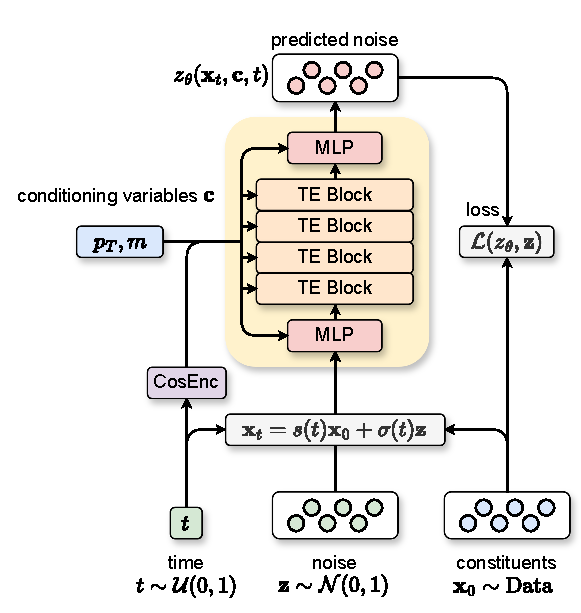
\includegraphics[width=0.65\textwidth]{Figures/jet_generation/pcjedi.pdf}
    \caption{The \pcjedi model architecture configured for training.}
    \label{fig:pcjedi}
\end{figure}

\subsubsection{Integration Solvers}

As with all diffusion models, to generate samples with \pcjedi, numerical integration is required to solve the reverse SDE or the probability flow ODE.
This complicates evaluation of the model, as sample quality can vary wildly depending on the solver used, and the number of integration steps taken.
Various numerical solvers for this task~\cite{NumericalSolutionStochastic} are compared.
The Euler-Maruyama (EM) method is used to solve the reverse SDE, and the DDIM sampler~\cite{DDIM} fourth-order Runge-Kutta and Euler methods are used for the probability flow ODE.
Equal step sizes were used for all solvers and negligible differences are observed between ODE solvers.

Generating higher quality samples with a diffusion model requires more integration steps, and thus longer generation times.
For these initial studies the focus was on quality rather than speed, so 200 integration steps were permitted for each jet.

\subsection{Results}

As a benchmark for performance, MPGAN~\cite{MPGAN}, a GAN trained on the same dataset, is used.
MPGAN generates the particle cloud with attributes $(\Delta\eta, \Delta\phi, \pt^\text{rel})$, where $\pt^\text{rel} = \pt / \ptjet$. Therefore, the outputs of \pcjedi are transformed to this format for comparison.
For evaluation, 50,000 jets per class are generated using MPGAN and \pcjedi with the different solvers.

Qualitative performance was assessed by visual inspection of the distributions of the generated jets compared to the JetNet30 test set.
For the distributions, we used the relative particle cloud kinematics, $\mpcrel$ and $\ptpcrel$, which were calculated using $\pt^\text{rel}$ for each constituent.
These distributions are shown in \Cref{fig:kinematics_gluon,fig:kinematics_top} for gluon and top jets.
Total $\ptpcrel$ is not always 1.0 due to the top 30 constituents' selection, though this is the maximum physical value.
All generative models struggle to capture the hard cut-off at 1.0 in but \pcjedi with DDIM solver shows the closest agreement.
Both \pcjedi models outperform MPGAN in reconstructing the top jet $\pt$ distribution, with similar performance in reproducing $\mpcrel$ for both jet types.
The bi-modal structure observed in top jet $\mpcrel$ arises from a phenomenon in boosted top jet reconstruction where the stable particles from the $b$-quark decay are not contained within the radius of the jet.
These top jets are referred to as \emph{uncontained} top jets, and they exhibit a 2-pronged structure and masses close to the mass of the $W$~boson.

\begin{figure}[hbpt]
    \centering
    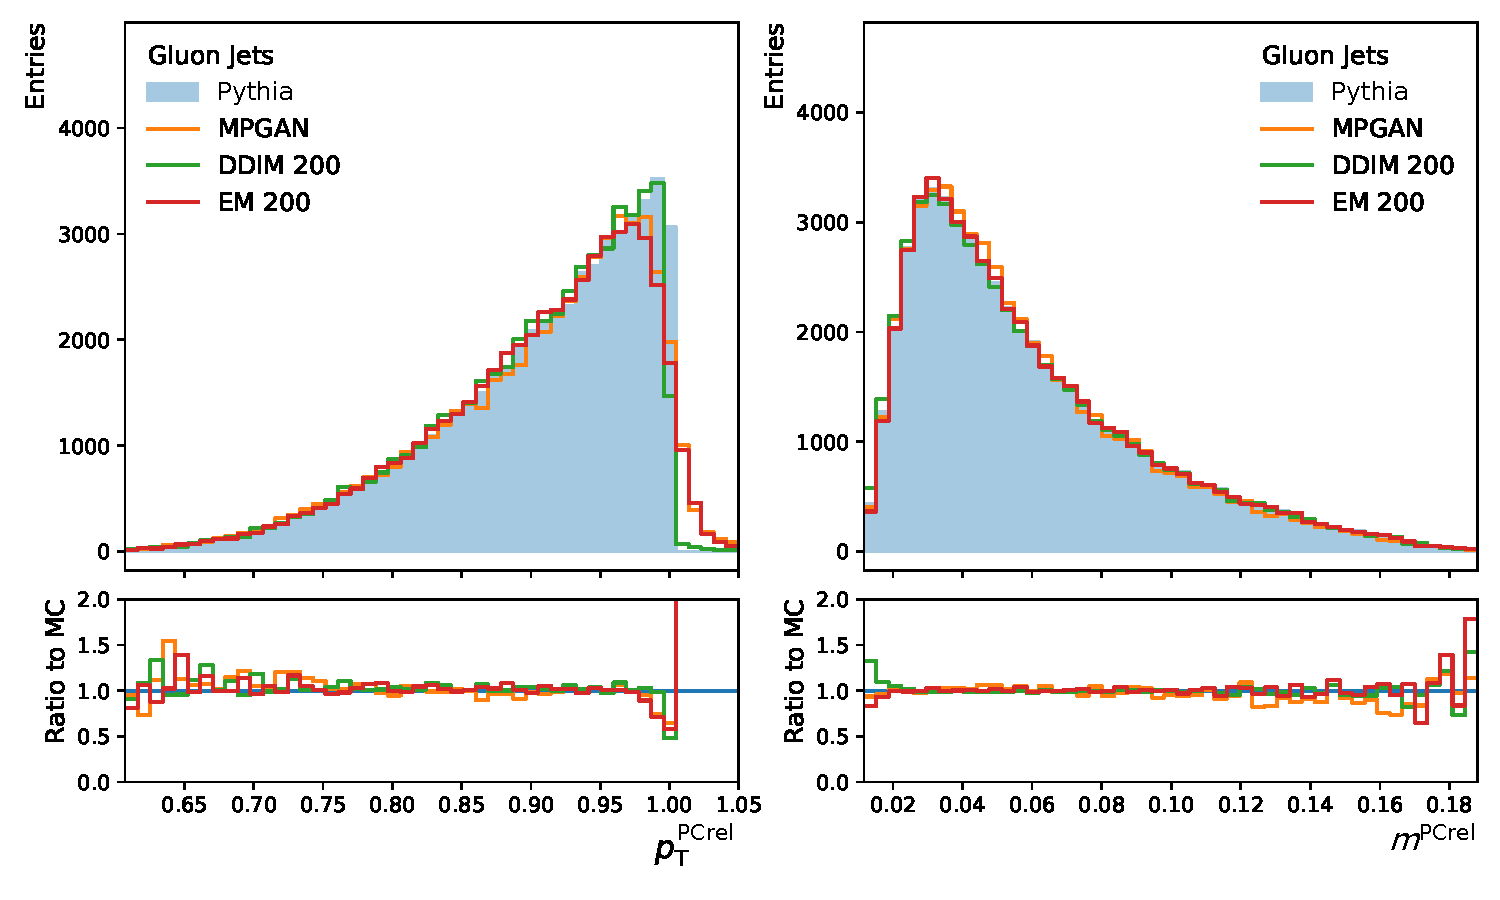
\includegraphics[width=.75\textwidth]{Figures/jet_generation/jedi/gluon/jet_features_rel.pdf}
    \caption{The relative transverse momentum (left) and invariant mass (right) of gluon jets generated with MPGAN and \pcjedi using the DDIM and EM solvers compared to the \pythia simulation. Calculated from the leading 30 \pt constituents using $\pt^\text{rel}$ instead of $\pt$.}
    \label{fig:kinematics_gluon}
\end{figure}

\begin{figure}[hbpt]
    \centering
    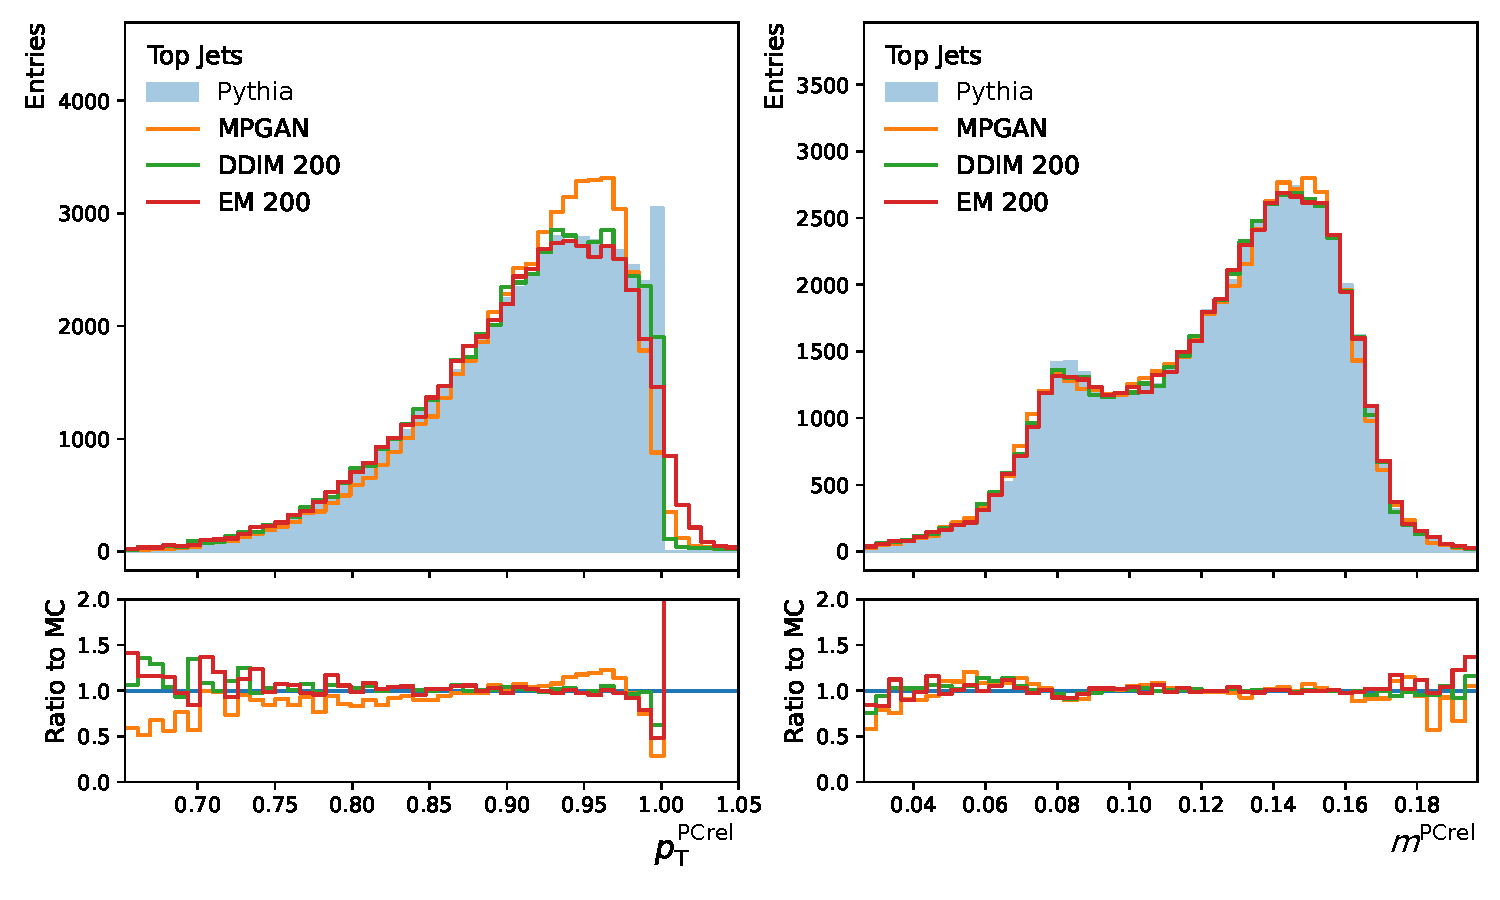
\includegraphics[width=.75\textwidth]{Figures/jet_generation/jedi/top/jet_features_rel.pdf}
    \caption{The relative transverse momentum (left) and invariant mass (right) of top jets generated with MPGAN and \pcjedi using the DDIM and EM solvers compared to the \pythia simulation. Calculated from the leading 30 \pt constituents using $\pt^\text{rel}$ instead of $\pt$.}
    \label{fig:kinematics_top}
\end{figure}

Crucial to the study of large-radius jets are the substructure variables $\tau_{21}$, $\tau_{32}$, and $\Dtwo$ as described in \Cref{sec:jet_substructure}\footnote{These variables are already normalized by the jet's total $\pt$, thus relative versions are unnecessary.}.
The subjettiness ratios $\tau_{21}$, $\tau_{32}$ in particular are essential for distinguishing top jets from gluon or quark jets.
Calculated for the generated particle cloud and compared to \pythia simulations, these variables are illustrated in \Cref{fig:substructure_gluon,fig:substructure_top}.
Both \pcjedi and MPGAN models accurately captured the $\text{D}_2$ distributions.
However, all models struggled with $\tau_{21}$ and $\tau_{32}$ especially for top jets, which exhibits a bi-modal structure due to the uncontained $b$-quark decay.

\begin{figure}[hbpt]
    \centering
    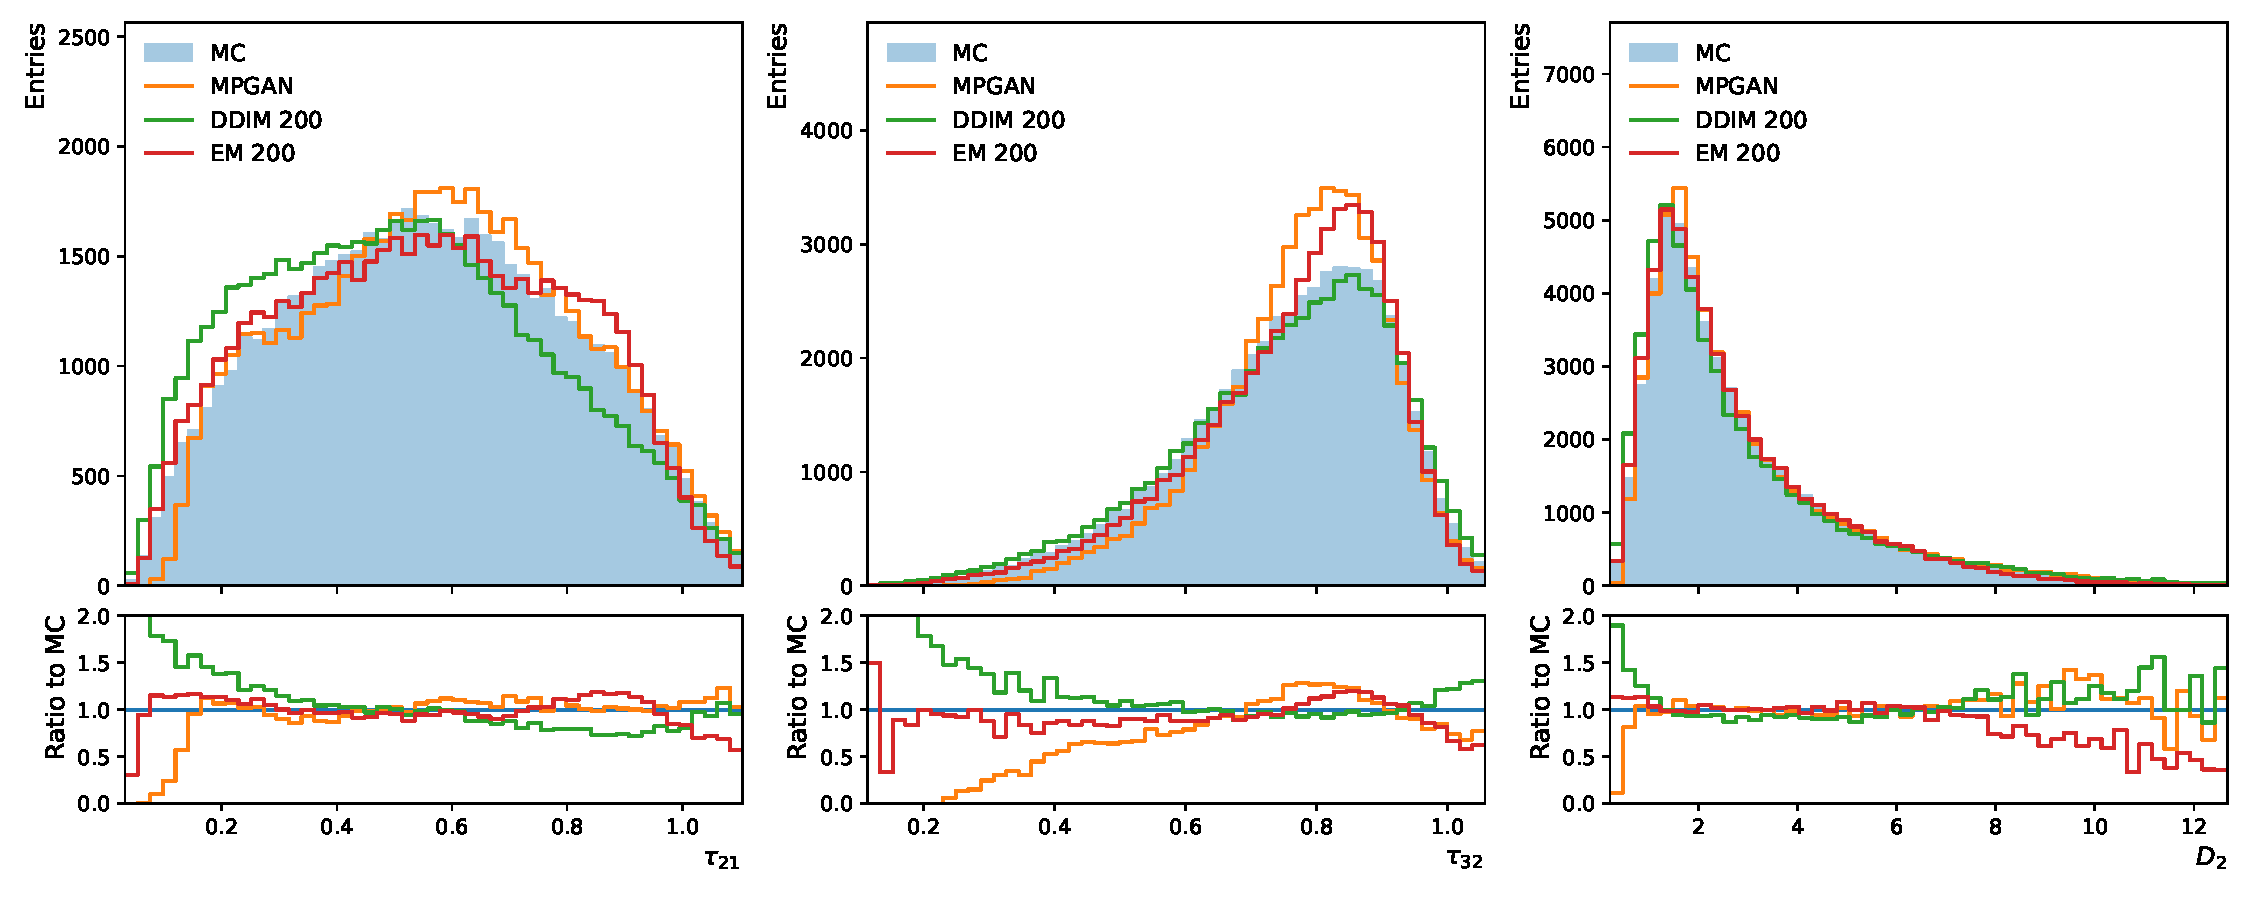
\includegraphics[width=1.\textwidth]{Figures/jet_generation/jedi/gluon/jet_substructure_rel.pdf}
    \caption{Substructure variables of gluon jets generated with MPGAN and \pcjedi using the DDIM and EM solvers compared to the \pythia.}
    \label{fig:substructure_gluon}
\end{figure}

\begin{figure}[hbpt]
    \centering
    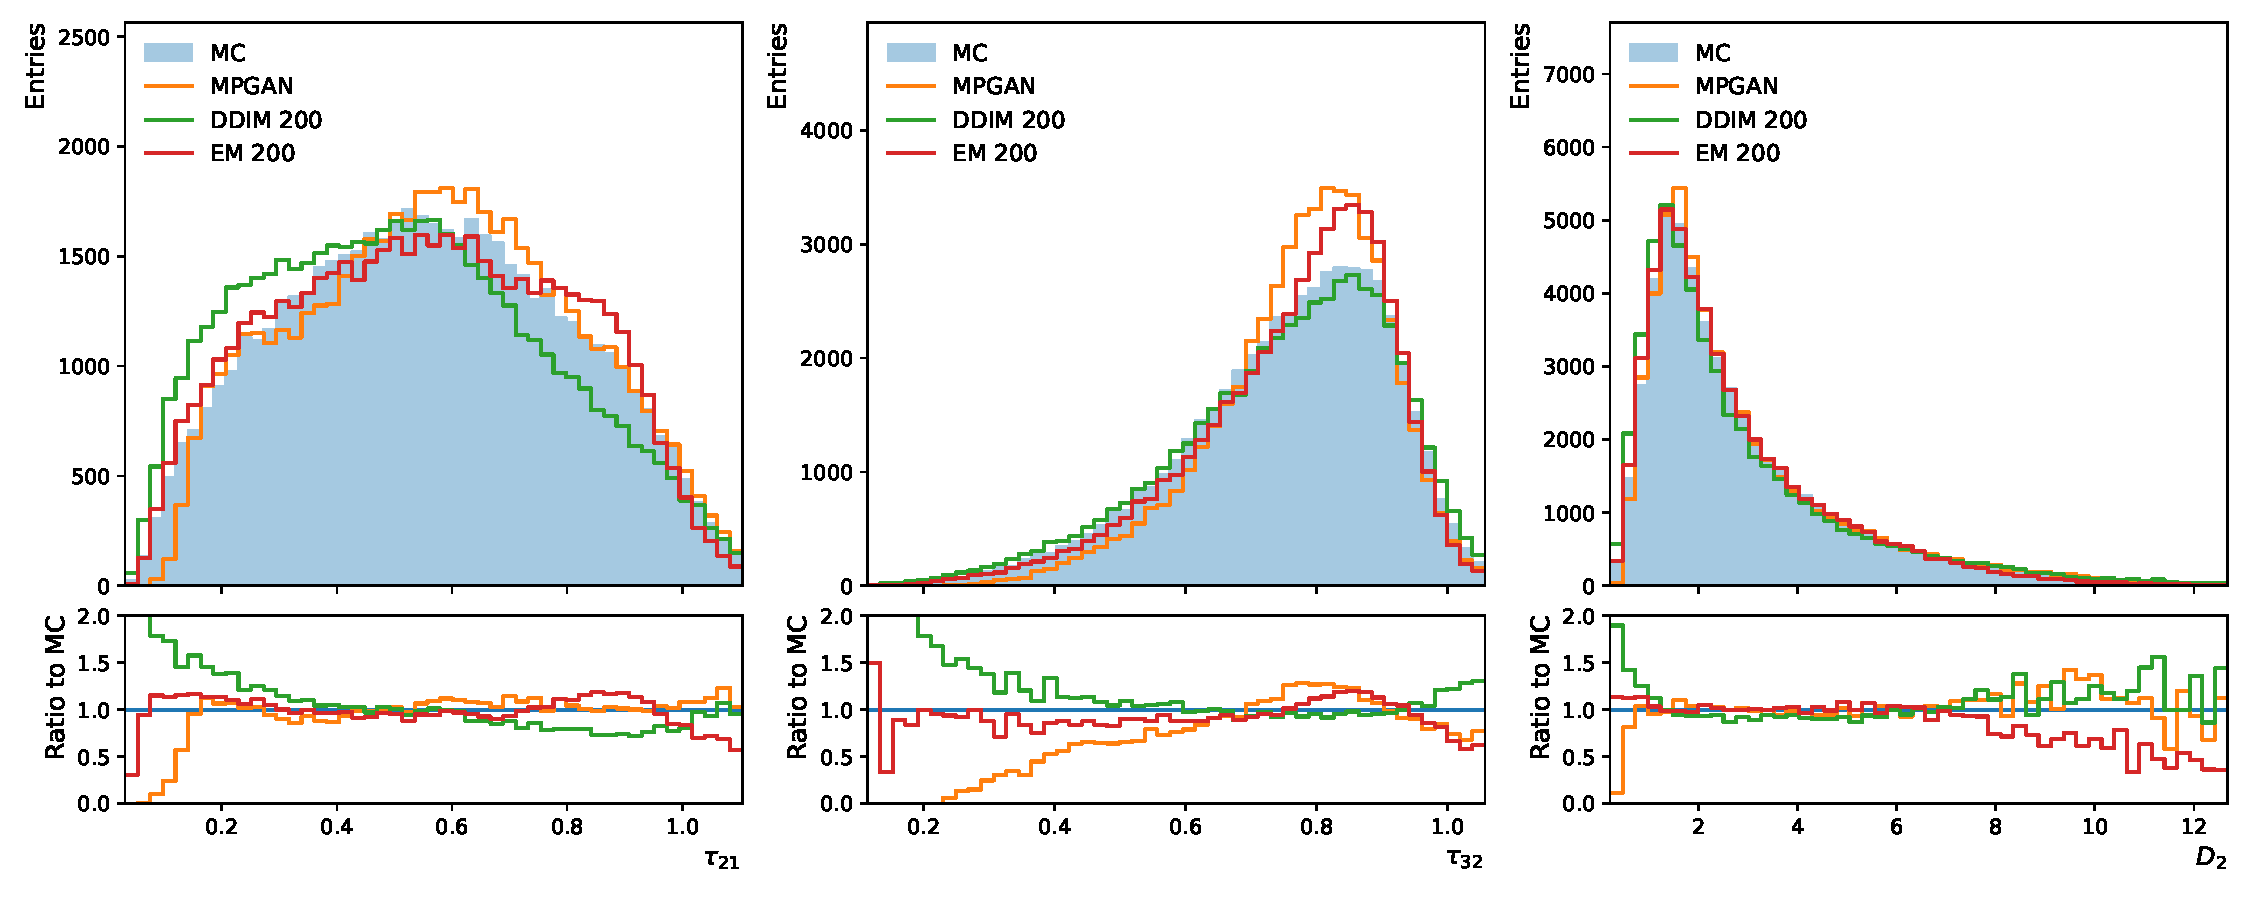
\includegraphics[width=1.\textwidth]{Figures/jet_generation/jedi/gluon/jet_substructure_rel.pdf}
    \caption{Substructure variables of top jets generated with MPGAN and \pcjedi using the DDIM and EM solvers compared to the \pythia simulation.}
    \label{fig:substructure_top}
\end{figure}

Quantitative metrics were derived following the methodology used in \textcite{MPGAN} whereby the Wasserstein-1 distance was calculated between the generated and \pythia jets, creating a $\text{W}_1$ score for each observable.
Uncertainties for these scores were derived using bootstrap sampling.
In addition to the distributions shown, we also calculated the $\text{W}_1$ score using the average of the first five Energy Flow Polynomials (EFPs)~\cite{EFP}, as these variables too are sensitive to the jet substructure.
Additionally, we computed the Fréchet ParticleNet distance (FPND), which compares the mean and standard deviation of the penultimate layer of the ParticleNet model for the \pythia and generated jets~\cite{MPGAN, ParticleNet}.
Lower limits for these values were calculated by comparing 50k jets from the training set to the test set, which captures the natrual variation in the data.
This allows us to compare the various methods quantitatively in \Cref{tab:combined_results}.
Based on these value, no one model is clearly superior.
\pcjedi with the EM sampler obtains the superior FPND score, but suffers greatly in the EFP distributions for top jets.
MPGAN outperforms \pcjedi in the $\Dtwo$ scores for gluon jets but not for top jets.
On average, it seems that the EM sampler is worse than the DDIM sampler, at least for the selected 200 integration steps, but the differences are not significant.
One crucial observation is how poorly all models perform on the subjetiness ratios with the ratio to \pythia for top jets, ranging from around 5 to 10 times higher than the MC-MC comparison.
This clearly indicates that the current methods are not sufficient for modelling the substructure of the large radius jets.

\begin{table}[tp]
    \centering
    \caption{Quantative comparison of the \pcjedi and MPGAN models for generating gluon and top jets.}
    \label{tab:combined_results}
    \renewcommand{\arraystretch}{1.5}
    \resizebox{\textwidth}{!}{%
        \begin{tabular}{llrrrrrr}
    \toprule
    Jet & Model        & FPND            & $\mathrm{W}_1^\mathrm{EFP}$ $(\times 10^{-6})$ & $\mathrm{W}_1^m$ $(\times 10^{-4})$ & $\mathrm{W}_1^{\tau_{21}}$ $(\times 10^{-3})$ & $\mathrm{W}_1^{\tau_{32}}$ $(\times 10^{-3})$ & $\mathrm{W}_1^{\Dtwo}$ $(\times 10^{-2})$ \\
    \midrule
    \multirow{4}{*}{Top}
        & \pythia      & $0.01$          & $8.07 \pm 3.51$                                & $3.23 \pm 1.07$                     & $2.01 \pm 0.74$                               & $2.90 \pm 1.59$                               & $1.16 \pm 0.29$                           \\ \cline{2-8}
        & \pcjedi-EM   & $\mathbf{0.15}$ & $35.61 \pm 4.92$                               & $13.64 \pm 3.21$                    & $4.55 \pm 1.16$                               & $\mathbf{16.05} \pm 1.31$                     & $\mathbf{2.08} \pm 0.40$                  \\
        & \pcjedi-DDIM & $0.28$          & $41.21 \pm 5.61$                               & $14.82 \pm 3.21$                    & $\mathbf{4.40} \pm 1.03$                      & $32.04 \pm 2.29$                              & $2.59 \pm 0.41$                           \\
        & MPGAN        & $0.36$          & $\mathbf{12.80} \pm 4.89$                      & $\mathbf{6.41} \pm 2.09$            & $6.61 \pm 0.92$                               & $17.41 \pm 2.78$                              & $3.40 \pm 0.63$                           \\
    \midrule
    \multirow{4}{*}{Gluon}
        & \pythia      & $0.01$          & $4.07 \pm 1.27$                                & $4.39 \pm 1.59$                     & $3.79 \pm 1.42$                               & $2.26 \pm 0.51$                               & $3.78 \pm 0.70$                           \\ \cline{2-8}
        & \pcjedi-EM   & $\mathbf{0.10}$ & $5.68 \pm 1.09$                                & $\mathbf{5.66} \pm 1.51$            & $12.48 \pm 0.98$                              & $\mathbf{13.32} \pm 0.96$                     & $10.20 \pm 1.04$                          \\
        & \pcjedi-DDIM & $0.12$          & $\mathbf{5.10} \pm 0.99$                       & $9.04 \pm 1.77$                     & $\mathbf{11.99} \pm 1.12$                     & $20.38 \pm 1.91$                              & $11.39 \pm 1.42$                          \\
        & MPGAN        & $0.13$          & $8.76 \pm 2.44$                                & $8.15 \pm 2.10$                     & $16.83 \pm 2.08$                              & $25.27 \pm 1.29$                              & $\mathbf{5.64} \pm 1.01$                  \\
    \bottomrule
\end{tabular}

    }
\end{table}

\subsection{Conclusion}

\pcjedi was the first model to generate particle clouds using a diffusion model, and while the results were promising, they were not state-of-the-art.
However, proving that the method could work was a significant step forward.
However, the time required to generate samples with diffusion models is a significant drawback, as it requires multiple forward passes compared to a single pass for a GAN\@.
The subsequent steps in this research would be to improve the model's performance and speed.

\FloatBarrier

\section{\pcdroid}

This section details the advancements made with \pcdroid, a successor to \pcjedi~\cite{PCDroid}.
The \pcdroid model exhibits marked improvements in speed and generation.
Leveraging an updated framework for diffusion models~\cite{ElucidatingDesignSpace}, enhanced diffusion sampling algorithms, and a novel transformer model, \pcdroid better balances performance and generation time.
Additionally, we explored using consistency distillation~\cite{ConsistencyModels} to even further reduce generation time.
\pcdroid achieves state-of-the-art performance on the benchmarks discussed in the previous section, notably surpassing both \pcjedi and MPGAN.
We also included much more elaborate timing studies to compare the various models against performing the showering using \pythia.
The code repository used in this work is publicly available~\cite{PCDroidCode}.

\subsection{Improved Diffusion Framework}

One of the main advancements in \pcdroid is the revised diffusion paradigm and configuration.
\pcdroid adheres to the EDM noise scheduler and network preconditioning as outlined by \textcite{ElucidatingDesignSpace}, discussed in \Cref{sec:diffusion_frameworks}.
This approach introduces several key modifications.

Firstly, the signal and noise rates are defined as $\gamma(t)=1$ and $\sigma(t)=t$.
This adjustment simplifies the forward SDE to
\begin{equation}
    \diff \x_t = \sqrt{2t} \diff \w_t,
\end{equation}
with the corresponding ordinary differential equation ODE similarly reducing to,
\begin{equation}
    \diff x_t = - t \score \diff t.
\end{equation}
As a result, the ODE solutions exhibit straighter trajectories, reducing truncation errors during generation compared to the previous variance-preserving method.
The primary advantage of this change is the ability to execute the reverse diffusion process in fewer steps.

Secondly, diffusion times are sampled during training specifically to target regions of the diffusion process where the model can gain the most information.
These diffusion times are used to scale the noise added to the input data.
Note that the diffusion time $t$ and noise rate $\sigma(t)$ can be used interchangeably, with $t$ extending beyond the range of 0 to 1, instead falling in the range $t = \sigma(t) \in [0, 80]$.
When $t$ is low, the magnitude of the artificial noise introduced into the samples is indistinguishable from the inherent stochasticity of the data.
Conversely, at high values of $t$, the input sample is almost entirely corrupted by noise, and the model can at most return the mean of the data distribution.
Log-normal sampling of the diffusion times, ${\log(t)\sim\mathcal{N}\left(-1.2, 1.2\right)}$, preferentially targets intermediate values where the model can learn the most.
This specific sampling distribution~\cite{ElucidatingDesignSpace} was observed to be advantageous for our tasks.

Thirdly, sophisticated skip and scaling connections are integrated into the network architecture.
The variables $c_\mathrm{in}(t)$, $c_\mathrm{out}(t)$, and $c_\mathrm{skip}(t)$ are all parameterized by $t$ and are combined for the denoised estimate as follows:
\begin{equation}
    x_\theta(\x, \cond, t) = c_\mathrm{out} f_\theta(c_\mathrm{in}\x, \cond, t) + c_\mathrm{skip}\x,
\end{equation}
where $f_\theta$ represents the raw prediction from the neural network.
Note that unlike \pcjedi, the target for the network is the true data sample $\x_0$ rather than the noise $\z$.
The skip connection permits $\x_t$ to bypass the network at low $t$, as the input is inherently closer to the target.
Due to the variance not being preserved during the diffusion process, these  scaling functions maintain the unit variance of the raw inputs and targets
for $f_\theta$.

We reuse the same dataset, JetNet30, as outlined in \Cref{sec:jetgen_data} for some experiments in this section.
However, most of the studies are performed using the extended JetNet150 dataset, which encompasses the same jets but with up to 150 constituents within the particle cloud.
This expanded dataset poses new challenges for the generative task, necessitating more intricate models and increased computational resources to manage the larger set size effectively.
Furthermore, we used all five jet types in JetNet150, rather than just the gluon and top jets.

\subsection{Model Architecture}

The general \pcdroid architecture and the training process is shown in \cref{fig:droid_arch_train}.

In addition to the preconditioning which comes from the EDM framework, the model has an additional MLP compared to \pcjedi which processes the conditional input before sending it to each sublayer.
This is primarily because the number of context variables increased to also include the jet azimuthal angle ($\phi$), the number of constituents (which was previously only implicitly included in the input set size), and the jet type (PID).
This last feature is significant because, whereas \pcjedi and MPGAN required separate models for each jet type, \pcdroid can generate all five jet types with a single conditional network.
Furthermore, the conditioning features represent the full jet kinematics, rather than just the net kinematics of the particle cloud.
This makes the generation a more challenging task, as it would have to learn the effects of truncating the particle cloud.

\begin{figure}[htpb]
    \centering
    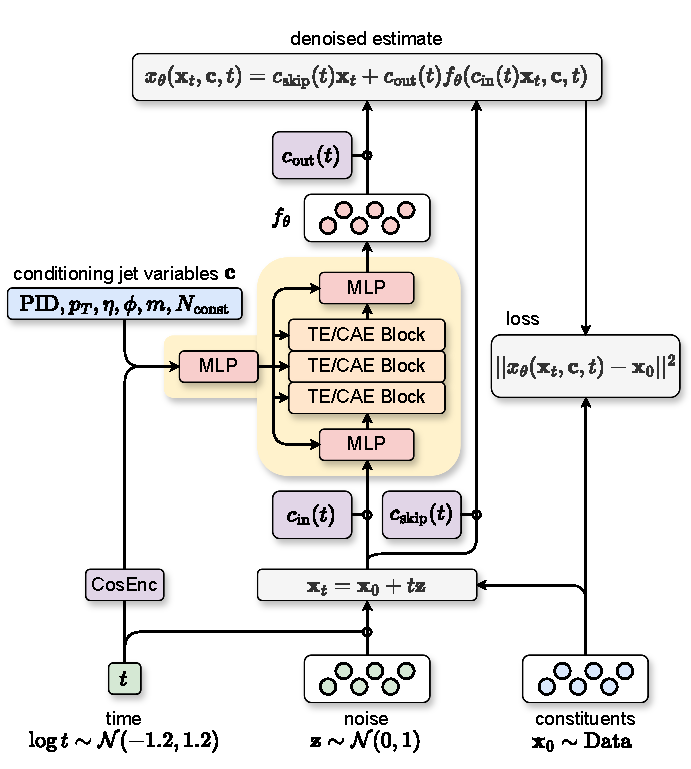
\includegraphics[width=0.6\textwidth]{Figures/jet_generation/pcdroid.pdf}
    \caption{The \pcdroid model architecture configured for training.}
    \label{fig:droid_arch_train}
\end{figure}

In \pcjedi, only TE Blocks with self-attention were studied, which, despite their high expressiveness, are computationally expensive.
The number of operations scales quadratically with the number of constituents $N_{const}$, i.e., $\mathcal{O}(N_{const}^2)$.
Given that diffusion models necessitate multiple network passes during generation, self-attention becomes a suboptimal choice for fast generation.
While this computational demand is manageable for models with 30 constituents, it becomes significantly impactful when scaling to 150 constituents.
Consequently, alongside the TE based model, we introduce the cross-attention encoder (CAE), which serves as a more efficient and memory-conserving permutation-equivariant network.

A schematic overview of the CAE Block is illustrated in \Cref{fig:cae_network}.
In a CAE Block, the input particle cloud updates a set of global tokens via multi-headed cross-attention, with the number of global tokens $N_{global}$ serving as a hyperparameter.
These tokens are then refined through a residual MLP and redistributed back to the point cloud using another cross-attention layer and residual MLP.
The full CAE is constructed by sequentially stacking multiple CAE Blocks, with the initial set of global tokens being fully learnable.
For $N_{global}=1$, the distribution attention operation employs a sigmoid function instead of softmax.
The CAE's attention operations scale with $\mathcal{O}(N_{const} \times N_{global})$.
The first attention operation effectively pools information from the point cloud into the global tokens. The second attention operation is inverted, and information from the updated global token are distributed back to the point cloud.

\begin{figure}[htpb]
    \centering
    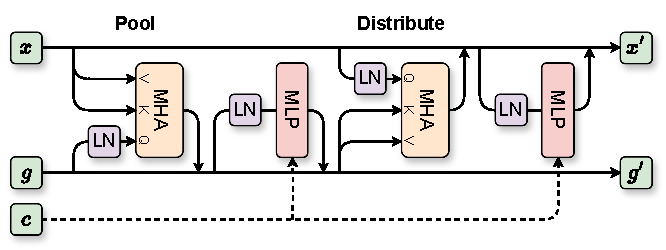
\includegraphics[width=0.8\textwidth]{Figures/jet_generation/CAEB.pdf}
    \caption{A single cross-attention encoder block updating both an input point cloud $x$ and global tokens $g$, using layer-norm (LN), multi-headed attention (MHA). Contextual information $c$ is injected into the network by concatenating to the inputs of the MLPs.}
    \label{fig:cae_network}
\end{figure}

To allow direct comparisons with \pcjedi, the optimizer, learning rate, scheduler, and the majority of hyperparameters remain unchanged.
The only notable adjustments, based on a minor hyperparameter scan, include reducing the number of encoder layers from four to three and using MSE loss for training.
For models with 150 constituents, the token dimension and the width of the MLP layers were doubled.
We trained two additional models utilizing CAE Blocks with $N_{global}=1$ and 16, on the 150 constituent dataset, employing the same training configuration, dimensions, and number of layers as the baseline model.

\subsubsection{Integration Solvers}

Another key development has been in the choice of integration solvers used during inference.
Several state-of-the-art algorithms have been studied and \pcdroid was designed to be compatible with the popular \textsc{K-Diffusion} library~\cite{KDiffusion}.
The most promising solvers include a fourth order linear multistep method (LMS)~\cite{ODEBook}, DPM-Solver-2~\cite{DPMSolverFastODE}, DPM-Solver++~\cite{DPMSolverFastSolver}, and DPM-Solver-2M~\cite{DPMSolverFastSolver}, and ancestral variants of these.
Furthermore, we experimented with non-uniform step sizes during generation, and found that systematically taking larger steps at the beginning of the denoising process and smaller steps towards the end improved the quality of the generated samples.

\subsection{Consistency Distillation}

Additionally, this work investigated the process of consistency distillation (CD) \cite{ConsistencyModels}, wherein a teacher network trains a student network to solve the reverse diffusion process in fewer steps, and in some cases enabling \textit{one-shot} generation.

The teacher network is a standard pre-trained diffusion model which together with a sampling method, defines a method to trace paths along the learned probability flow ODE.
During distillation, the weights of the teacher network are frozen, and a student network is trained to map all points sampled along a same ODE trajectory a common target.
To prevent the student model from collapsing into a constant function, a boundary condition is enforced such that the student must become an identity map as the diffusion time approaches zero.
The same skip connections used in the \pcdroid model are employed to enforce this.
This boundary condition ensures the global minimum of the training loss was achieved only when the student network mapped each point of the ODE trajectory to its endpoint.

Initially, the student model is initialized with the same parameter values as the teacher model.
During training, the diffusion time is sampled, the input is corrupted using the same schedule as before, and then the teacher model is used to take a single step along the ODE.
These two adjacent points on the ODE are each passed through the student network, and the student is trained to minimize the mean squared distance between its two outputs.
To stabilize training, the student network was duplicated into an online and target network, a practice common in deep reinforcement learning \cite{PlayingAtariDeep, ContinuousControlDeep, ImplicitQuantileNetworks}.
Gradients propagated only through the online network, which always processed the ODE sample with the larger $t$.
After each iteration, the target network was synced with the student network using an EMA of the parameters.

Although both are distillation methods, CD differs from progressive distillation models (PD) \cite{ProgressiveDistillationFast}.
In progressive distillation, new models are iteratively trained to predict the amount of noise removed in $N$ steps of the previous model.
This iterative process reduces the overall number of steps required with each new model, thereby resulting in faster generation times.
Unlike CD, PD does not require information about the ODE trajectories, only the total amount of noise removed after $N$ steps.

\subsection{Unconditional Generation}

\pcdroid is trained as a conditional generative model, with the jet kinematics $(\pt, \eta, m)$, the number of constituents ($N_{const}$), and the PID used as conditions.
We can marginalize the conditional variables using a second generative model to allow for unconditional generation.
As this is a low-dimensional vector, we trained NFs for this task.
This approach is preferable to explicitly unconditional models as it logically segments the learning process.

Standard use cases would still demand control over the jet type, so
one flow (Flow-$\p$) is trained to learn the probability density $p(\pt, \eta, m, N_{const} |\textrm{PID})$.
A second flow (Flow-$N$) is trained to learn the probability density $ p(N_{const}|\pt, \eta, m, \textrm{PID}) $.
This second flow demonstrates how \pcdroid can be used as a surrogate fast simulator, especially when the parton type and kinematics are known, but the number of particles in the final jet is not.
As the transformer denoises all input tokens, the number of constituents is always required at generation time.
This number is correlated to many jet properties, necessitating a normalizing flow rather than simply sampling from a Poisson distribution.

Both flows are trained with a maximum log-likelihood objective and consist of five transformation layers using rational quadratic splines~\cite{NeuralSplineFlows}.
Coupling layers are used in Flow-$\p$, while none are needed for the one-dimensional transformation Flow-$N$.
For both flows, a dequantization step simplifies the learning of the $N_{const}$ distribution; at inference time, the generated value is rounded to the nearest integer.
The Adam optimizer~\cite{Adam} with default settings and a cosine learning rate is used.
Given the relatively simple nature of these distributions, near-perfect performance is achieved using only four layers and 100k learnable parameters.

\subsection{Results on JetNet30}

We compared the \pcdroid, \pcjedi, and MPGAN models on the JetNet30 dataset using the same distributions and metrics as before.
This study utilized \pcdroid samples generated under the fully conditional regime.
Performance comparison revealed minimal differences between jets conditioned on the training set kinematics and those conditioned on the flow outputs.

We test a wide variety of integration solvers in the generation stage for \pcjedi.
We studied the trade-off between the quality of generated jets and the number of neural function evaluations (NFE) to determine the optimal solver and step size.
The comparison focused on the FPND, $\mathrm{W}_1^M$, and $\mathrm{W}1^{\tau{32}}$ metrics, given the latter's difficulty in previous studies.
For \pcjedi we used the results using the Euler-Maruyama sampler at 200 NFE.
From \cref{fig:metrics_vs_steps-30}, we observe most solvers saturating around 100 NFE.
We generated samples with \pcdroid using Heun and HeunSDE methods~\cite{ElucidatingDesignSpace}, DPM2~\cite{DPMSolverFastODE}, DPM2 with ancestral sampling (DPM2A), DPM++2M~\cite{DPMSolverFastSolver}, and LMS~\cite{ODEBook}
Although no method was clearly superior, the LMS solver generally performed best across most metrics, and was thus used at 100 NFE for all \pcdroid results in the following sections.
Additionally, \pcdroid outperformed MPGAN with as few as 20 steps for most solvers.

\begin{figure}[tb]
    \centering
    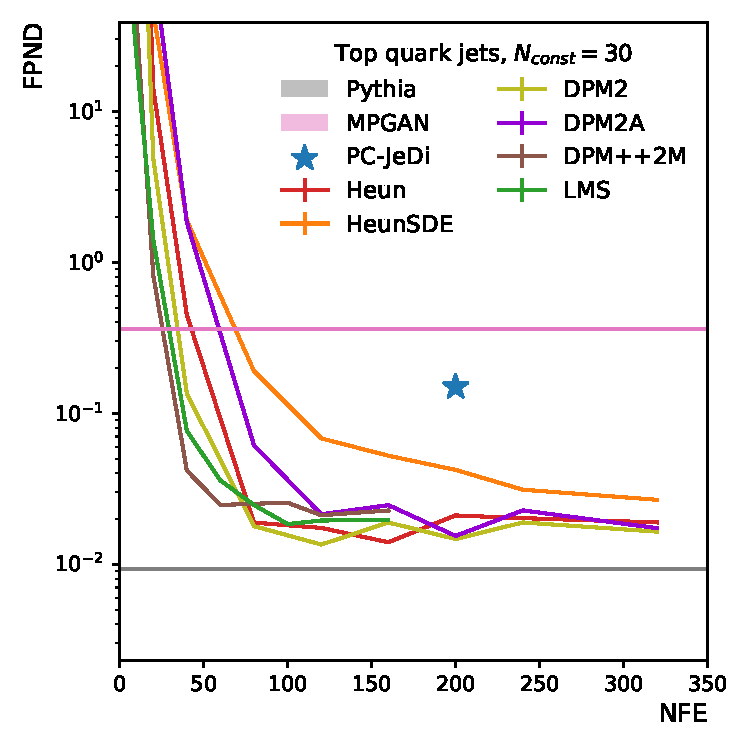
\includegraphics[width=0.32\textwidth]{Figures/jet_generation/droid/30/metrics_vs_steps/t/t_fpnd.pdf}
    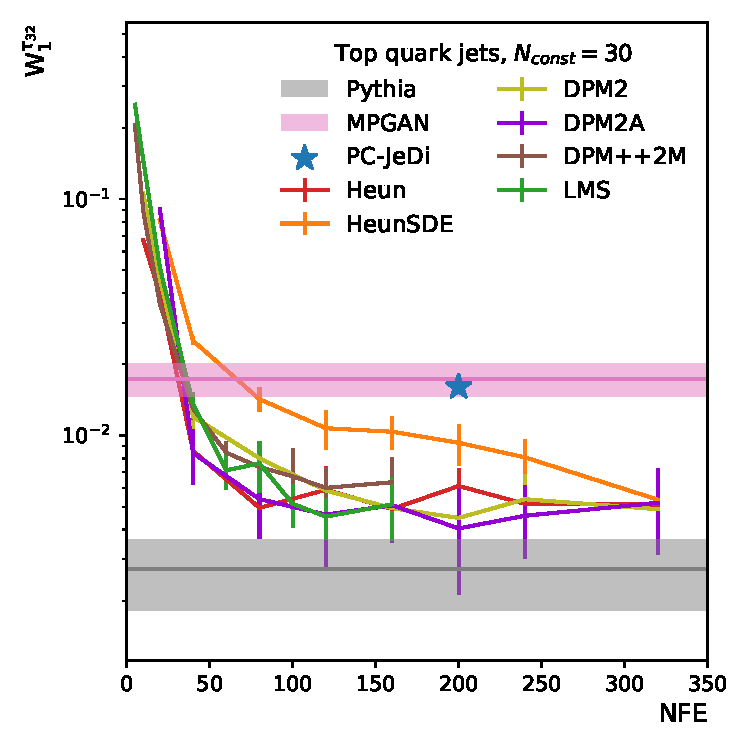
\includegraphics[width=0.32\textwidth]{Figures/jet_generation/droid/30/metrics_vs_steps/t/t_w1_tau_32.pdf}
    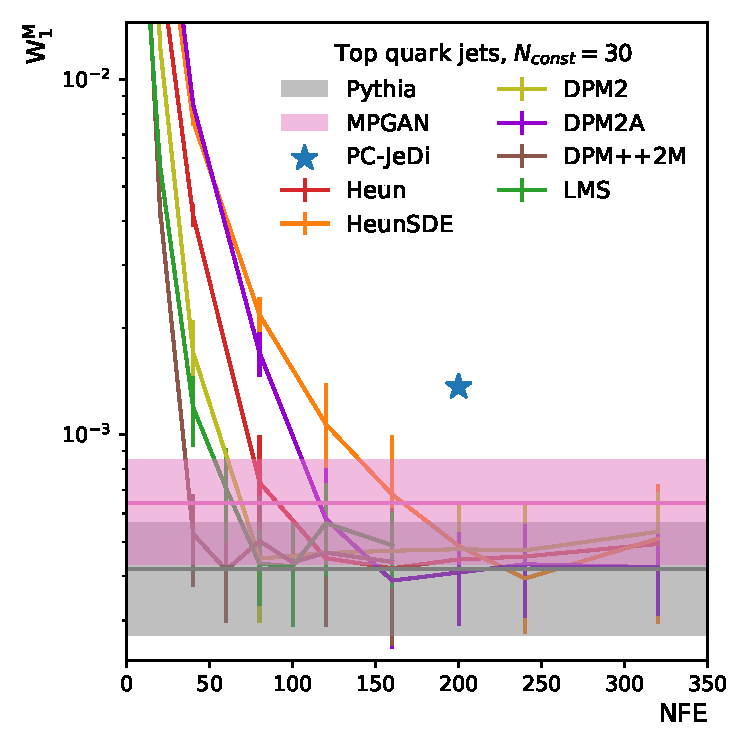
\includegraphics[width=0.32\textwidth]{Figures/jet_generation/droid/30/metrics_vs_steps/t/t_w1m.pdf}
    \caption{Performance as measured by FPND (left), W$_1^{\tau_{32}}$ (middle), and W$_1^m$ (right) as a function of the NFE used during generation for the \pcdroid model for top jets with up to 30 constituents.}
    \label{fig:metrics_vs_steps-30}
\end{figure}

Effectively modelling the kinematics of individual constituents is essential for jet generation.
\Cref{fig:const-pt_dist-30} illustrates the \pt distributions of the leading, fifth leading, and twentieth leading constituents of the generated top and gluon jets, as represented by \pcdroid and \pcjedi.
\pcdroid shows better alignment with \pythia compared to \pcjedi across all constituents, especially in the distribution tails.

\begin{figure}[htpb]
    \centering
    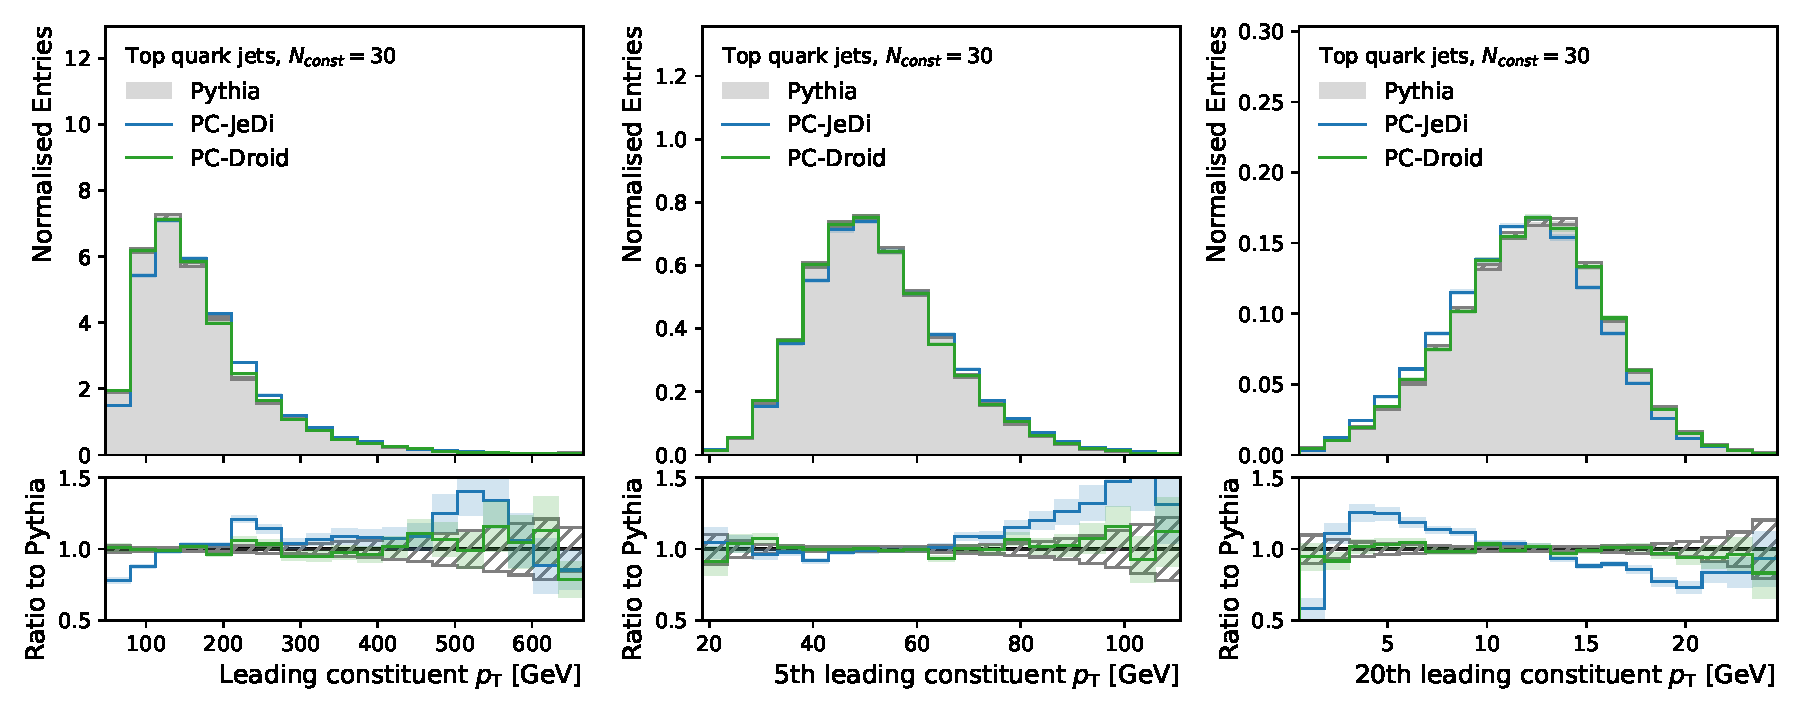
\includegraphics[width=0.99\textwidth]{Figures/jet_generation/droid/30/csts/t/100/t_leading_constituents.pdf} \\
    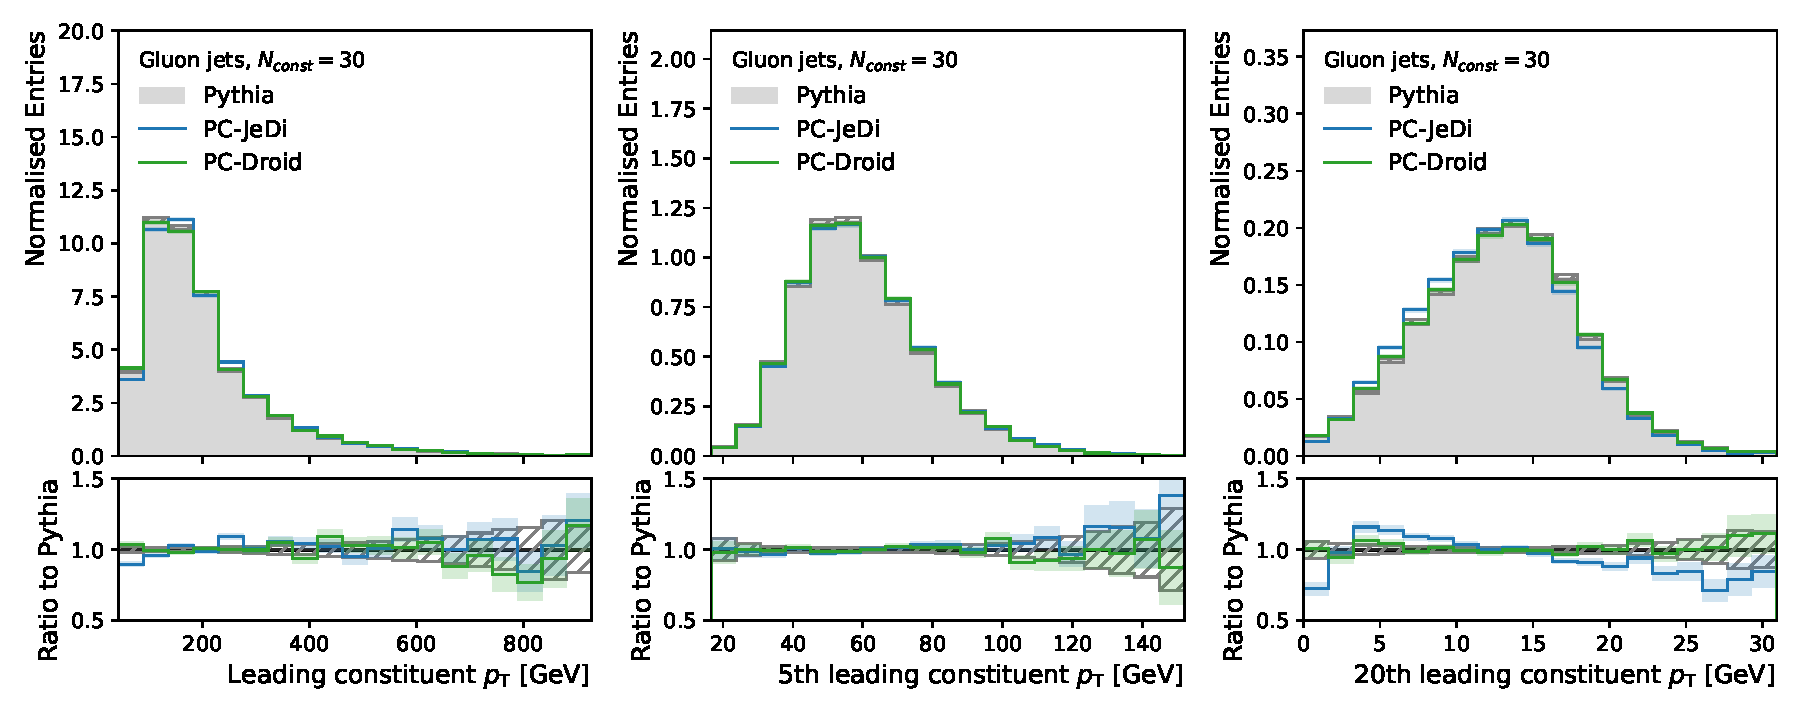
\includegraphics[width=0.99\textwidth]{Figures/jet_generation/droid/30/csts/g/100/g_leading_constituents.pdf}
    \caption{Comparison of \pt distributions of the leading, fifth leading, and twentieth leading constituents of the generated top and gluon jets with up to 30 constituents.}
    \label{fig:const-pt_dist-30}
\end{figure}

Next, we examine the substructure variable distributions of the generated jets and their correlations, essential for jet tagging.
We focus on top jets due to their complex substructure, which has proven challenging to model.
\Cref{fig:hlvs-30} shows that \pcdroid significantly improves $\tau_{32}$ modelling compared to \pcjedi and aligns excellently with \pythia simulations for all other substructure variables.

\begin{figure}[htpb]
    \centering
    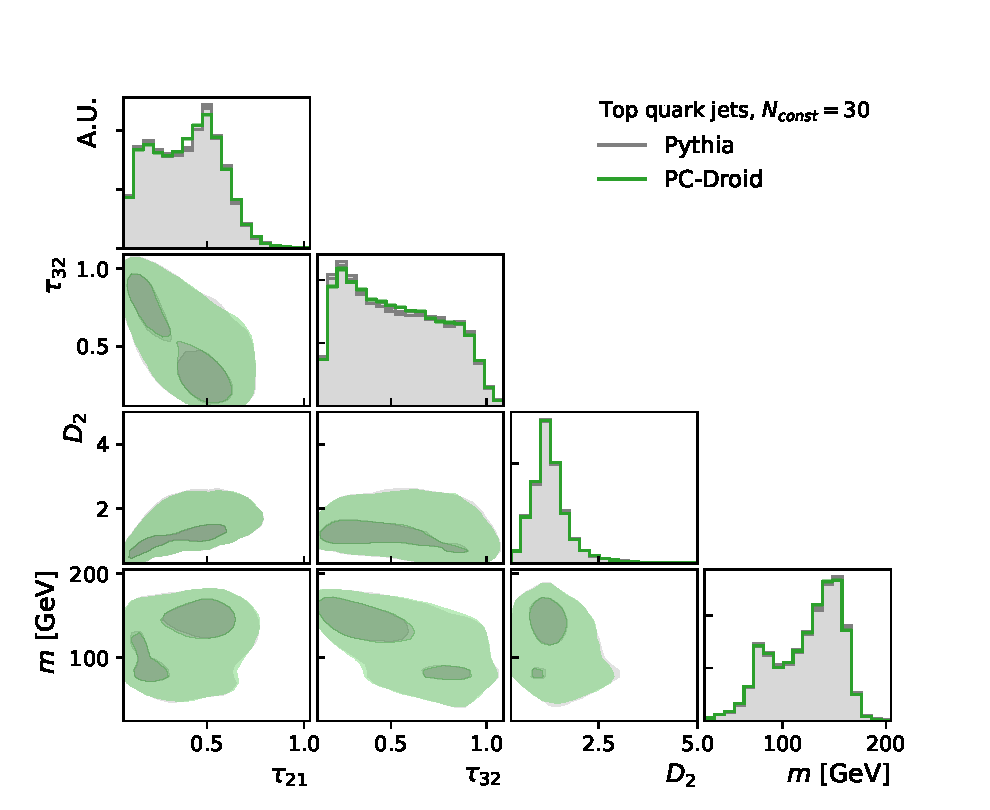
\includegraphics[width=0.49\textwidth]{Figures/jet_generation/droid/30/hlvs/t/100/hlv_corr_PC-Droid.pdf}
    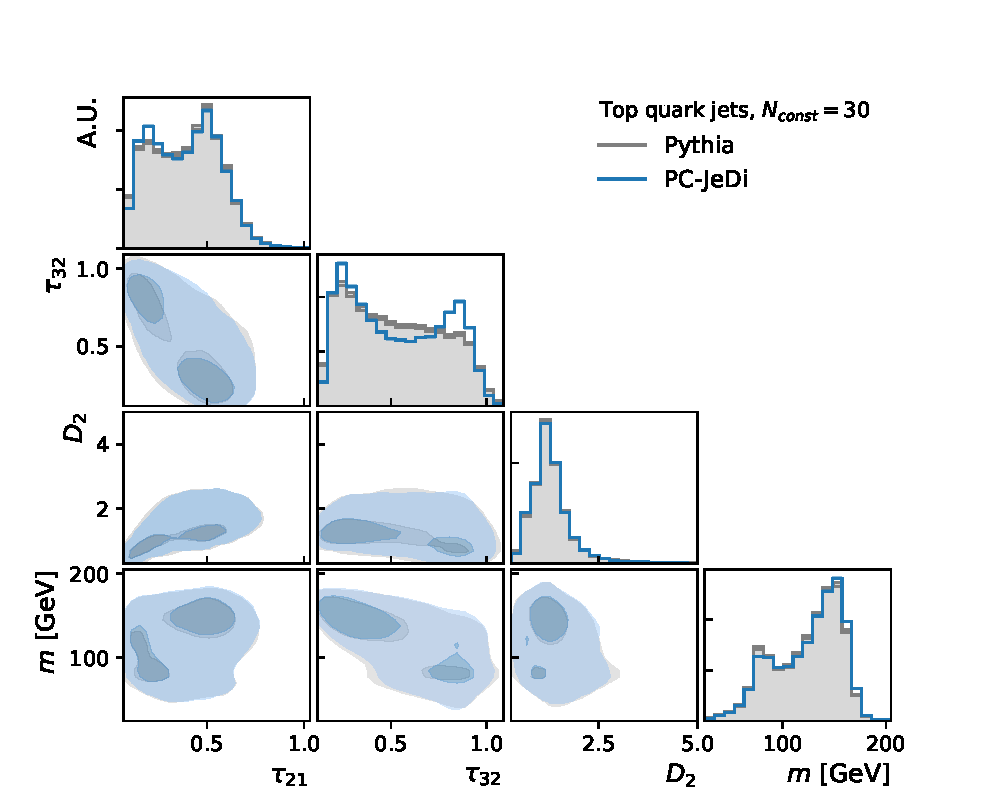
\includegraphics[width=0.49\textwidth]{Figures/jet_generation/droid/30/hlvs/t/100/hlv_corr_PC-Jedi.pdf}
    \caption{
        Mass and substructure distributions of the generated top jets with up to 30 constituents.
        The diagonal consists of the marginals of the distributions and the off-diagonal elements contain the joint distributions.
    }
    \label{fig:hlvs-30}
\end{figure}

The generation performance is summarized in~\cref{tab:30_table} for gluon and top jets.
The $\mathrm{W_1^P}$ score describes the average Wasserstein-1 distance between the marginal distributions of the generated and \pythia constituent kinematics.
Particularly in FPND, \pcdroid surpasses all other methods in all metrics, reaching the intra MC-MC comparison limits in the subjettiness ratios for gluons and $\mathrm{W_1^{\Dtwo}}$ for both jet types.

\begin{table}[tp]
    \centering
    \caption{Comparison of generative models on top and gluons with up to 30 constituents. Lower is better.}
    \label{tab:30_table}
    \renewcommand{\arraystretch}{1.5}
    \resizebox{\textwidth}{!}{%
        \begin{tabular}{llrrrrrrr}
    \toprule
    Jet & Model    & FPND            & $\mathrm{W_1^P}$ $(\times 10^{-4})$ & $\mathrm{W}_1^\mathrm{EFP}$ $(\times 10^{-6})$ & $\mathrm{W}_1^m$ $(\times 10^{-4})$ & $\mathrm{W}_1^{\tau_{21}}$ $(\times 10^{-3})$ & $\mathrm{W}_1^{\tau_{32}}$ $(\times 10^{-3})$ & $\mathrm{W}_1^{\Dtwo}$ $(\times 10^{-2})$ \\
    \midrule
    \multirow{4}{*}{Top}
        & \pythia  & $0.01$          & $3.98 \pm 1.27$                     & $8.07 \pm 3.51$                                & $3.23 \pm 1.07$                     & $2.01 \pm 0.74$                               & $2.90 \pm 1.59$                               & $1.16 \pm 0.29$                           \\ \cline{2-9}
        & \pcdroid & $\mathbf{0.02}$ & $\mathbf{5.02 \pm 1.59}$            & $\mathbf{11.59 \pm 3.29}$                      & $\mathbf{4.27 \pm 1.39}$            & $\mathbf{2.91 \pm 1.09}$                      & $\mathbf{5.14 \pm 1.06}$                      & $\mathbf{1.26 \pm 0.33}$                  \\
        & PC-JeDi  & $0.15$          & $12.07 \pm 2.01$                    & $35.61 \pm 4.92$                               & $13.64 \pm 3.21$                    & $4.55 \pm 1.16$                               & $16.05 \pm 1.31$                              & $2.08 \pm 0.40$                           \\
        & MPGAN    & $0.36$          & $21.73 \pm 2.02$                    & $12.80 \pm 4.89$                               & $6.41 \pm 2.09$                     & $6.61 \pm 0.92$                               & $17.41 \pm 2.78$                              & $3.40 \pm 0.63$                           \\
    \midrule
    \multirow{4}{*}{Gluon}
        & \pythia  & $0.01$          & $3.54 \pm 1.19$                     & $4.07 \pm 1.27$                                & $4.39 \pm 1.59$                     & $3.79 \pm 1.42$                               & $2.26 \pm 0.51$                               & $3.78 \pm 0.70$                           \\ \cline{2-9}
        & \pcdroid & $\mathbf{0.01}$ & $\mathbf{3.66 \pm 1.07}$            & $\mathbf{4.13 \pm 1.61}$                       & $\mathbf{4.48 \pm 1.47}$            & $\mathbf{2.89 \pm 0.80}$                      & $\mathbf{1.99 \pm 0.51}$                      & $\mathbf{3.52 \pm 1.33}$                  \\
        & PC-JeDi  & $0.10$          & $5.83 \pm 1.44$                     & $5.68 \pm 1.09$                                & $5.66 \pm 1.51$                     & $12.48 \pm 0.98$                              & $13.32 \pm 0.96$                              & $10.20 \pm 1.04$                          \\
        & MPGAN    & $0.13$          & $10.26 \pm 1.51$                    & $8.76 \pm 2.44$                                & $8.15 \pm 2.10$                     & $16.83 \pm 2.08$                              & $25.27 \pm 1.29$                              & $5.64 \pm 1.01$                           \\
    \bottomrule
\end{tabular}

    }
\end{table}

\FloatBarrier

\subsection{Results on JetNet150}

The JetNet150 dataset poses a more challenging task, both due to the increased number of constituents and the inclusion of all five jet types.
For plots however, we focus on top jets, as they are the most challenging to model, but we derive metrics for all types.
We compare marginals of the leading, fifth leading, and twentieth leading constituents of the generated jets compared to \pythia.
This is shown in \Cref{fig:const-pt_dist-150}.
We found that almost all methods were able to perform sufficiently well in this task.
Substructure distributions are displayed in Figure \Cref{fig:hlvs-150-marginals}.
A comparison between in the high level correlations between the transformer and CAE-1 models are shown in \Cref{fig:hlvs-150}.
Both models accurately capture jet mass and $\Dtwo$, though CAE-1 exhibits slightly diminished performance in subjettiness ratios.

MPGAN was never developed 150 constituents so as benchmarks for this dataset, we compare to two other deep generative models: FPCD~\cite{FPCD} and EPiC-GAN~\cite{EPICGAN}.

FPCD is a similar diffusion model which was developed concurrently with \pcdroid.
It too trains on all jet types simultaneously, employs a second model for generating conditions, and can produce jets with up to 150 constituents. It uses different network layers, diffusion schedule, and framework compared to \pcdroid.
FPCD jointly trains a second diffusion to generate the kinematics and $N_{const}$ of the jets given the PID.
We argue however that this an orthogonal task and does not need to share the same layers or noise seed.
It also means that for unconditional generation, FPCD requires two separate numerical integrations.
Similar to how we apply CD, FPCD was progressively distilled (PD) to a single step.

EPiC-GAN is a GAN model using specificially designed layers.
Rather than using conventional message passing, EPiC layers pool information to a global vector, then concatenate this to the input the node updates in the next layer.
It is essentailly a repeated implementation of a deep set and also shares similarities with the CAE model.
In EPiC-GAN a kernel-density estimator is used to model the number of constituents, which is a conditional parameter of the generation and correlated to the jet invariant mass and \pt.
However, the KDE does not take into account correlations between the number of constituents and the kinematics of the jet.

We evaluate both the original transformer-based model and CAE networks with 1 and 16 global tokens, labelled CAE-1 and CAE-16, respectively.
We provide a quantitative comparison between the performance of the \pcdroid and other models in \cref{tab:perf-150}.
All models here are run in the conditional mode.
\pcdroid with the self attention network displays superior performance in all metrics on all jet types wherever there is notable separation between models.
Where performance is saturated, the CAE-1 or CAE-16 models are comparable to the transformer model.
The LMS sampling method at 100 NFE yielded similarly optimal results for both networks and was used to derive all following results.

\begin{figure}[tb]
    \centering
    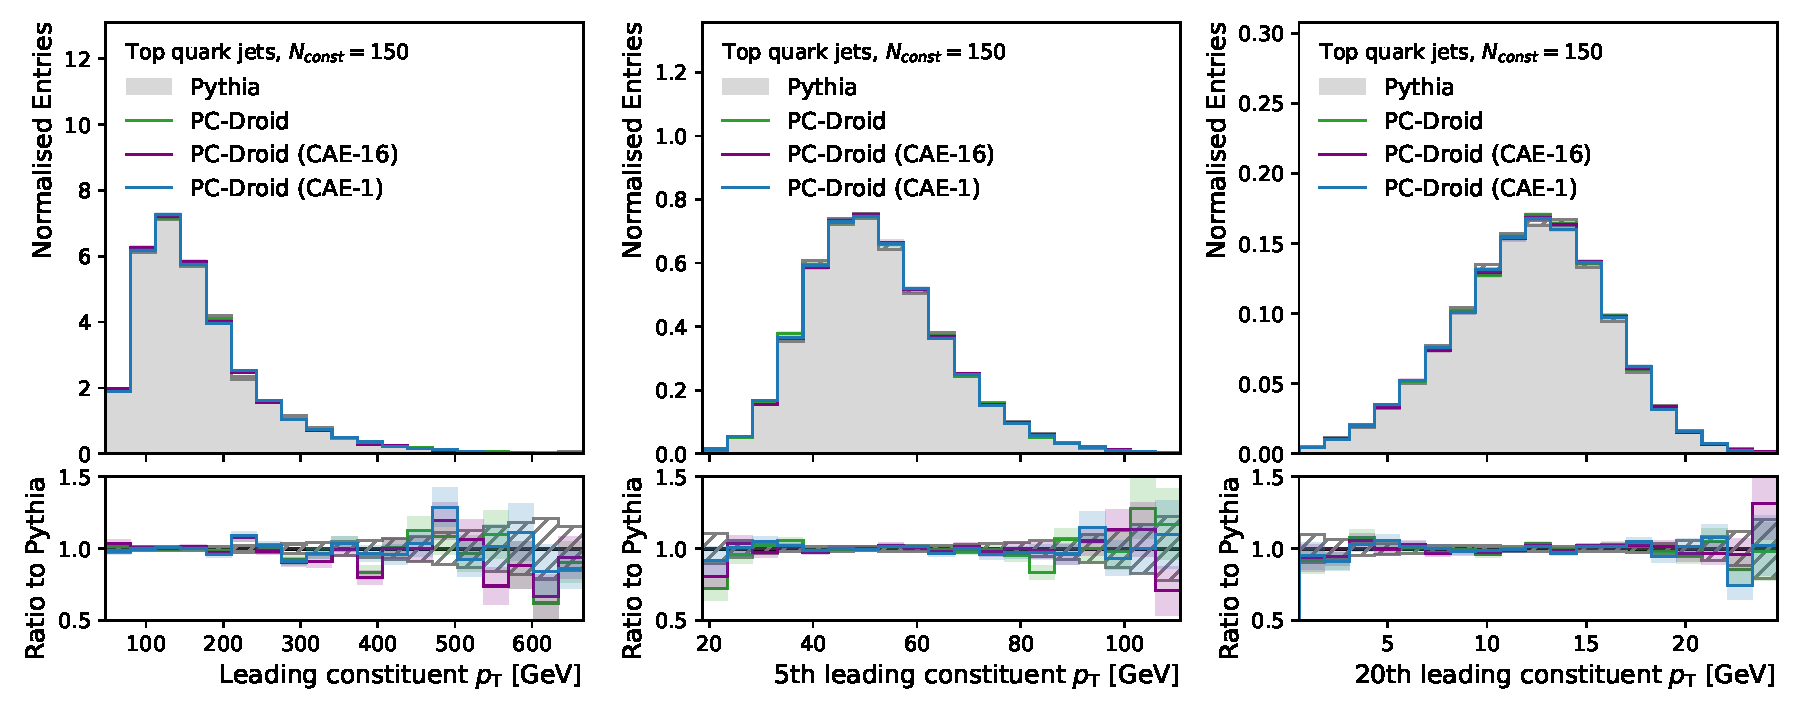
\includegraphics[width=0.99\textwidth]{Figures/jet_generation/droid/150/csts/t/100/t_leading_constituents.pdf}
    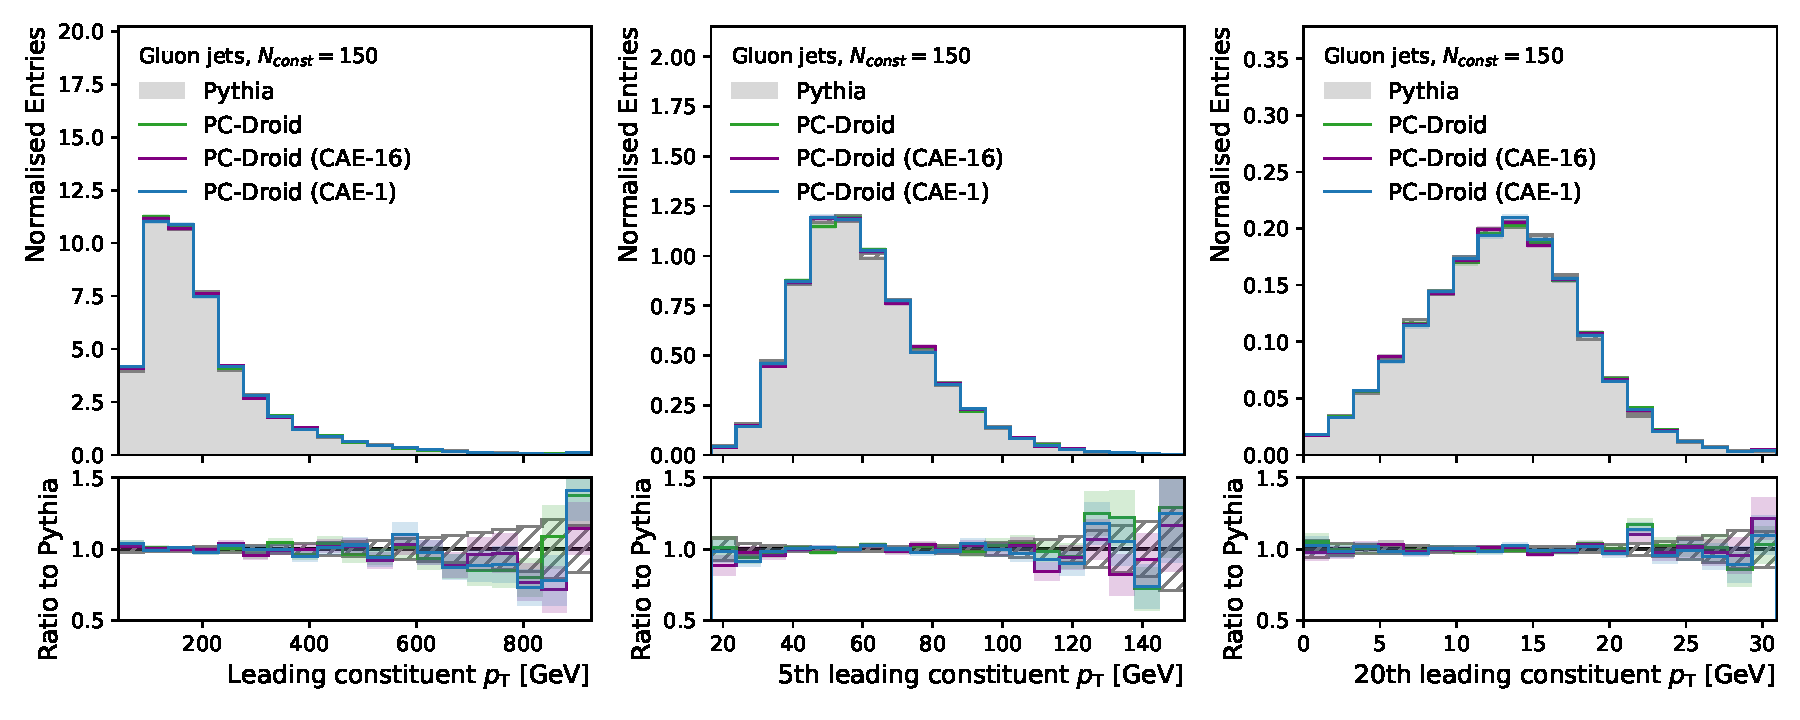
\includegraphics[width=0.99\textwidth]{Figures/jet_generation/droid/150/csts/g/100/g_leading_constituents.pdf}
    \caption{Comparison of \pt distributions of the leading, fifth leading, and twentieth leading constituents of the generated top and gluon jets with up to 150 constituents.
    }
    \label{fig:const-pt_dist-150}
\end{figure}

\begin{figure}[tb]
    \centering
    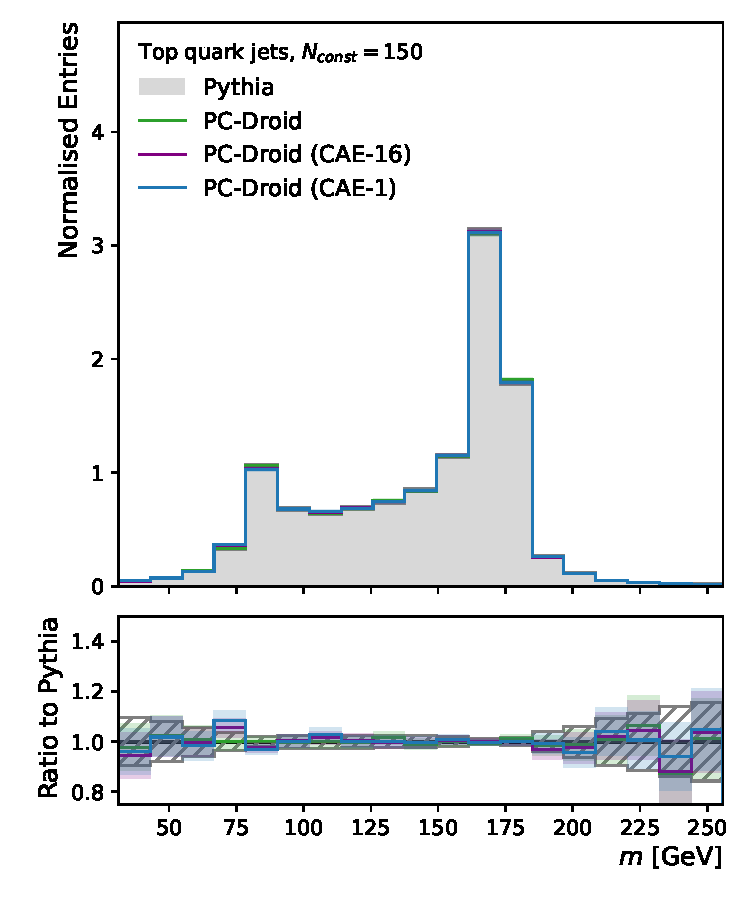
\includegraphics[width=0.33\textwidth]{Figures/jet_generation/droid/150/hlvs/t/100/mass.pdf}
    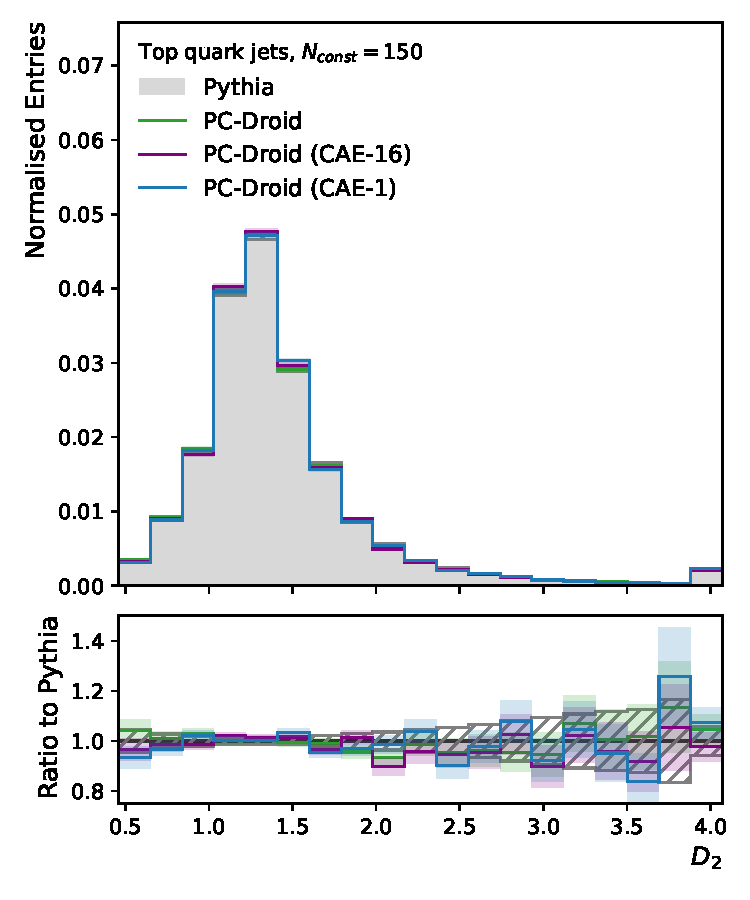
\includegraphics[width=0.33\textwidth]{Figures/jet_generation/droid/150/hlvs/t/100/d2.pdf} \\
    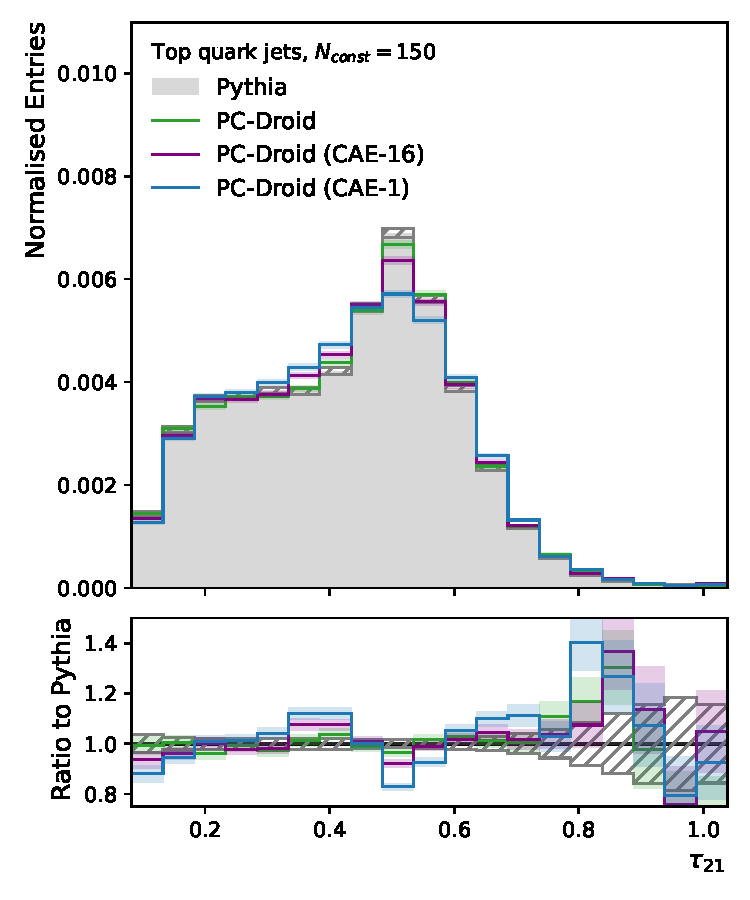
\includegraphics[width=0.33\textwidth]{Figures/jet_generation/droid/150/hlvs/t/100/tau_21.pdf}
    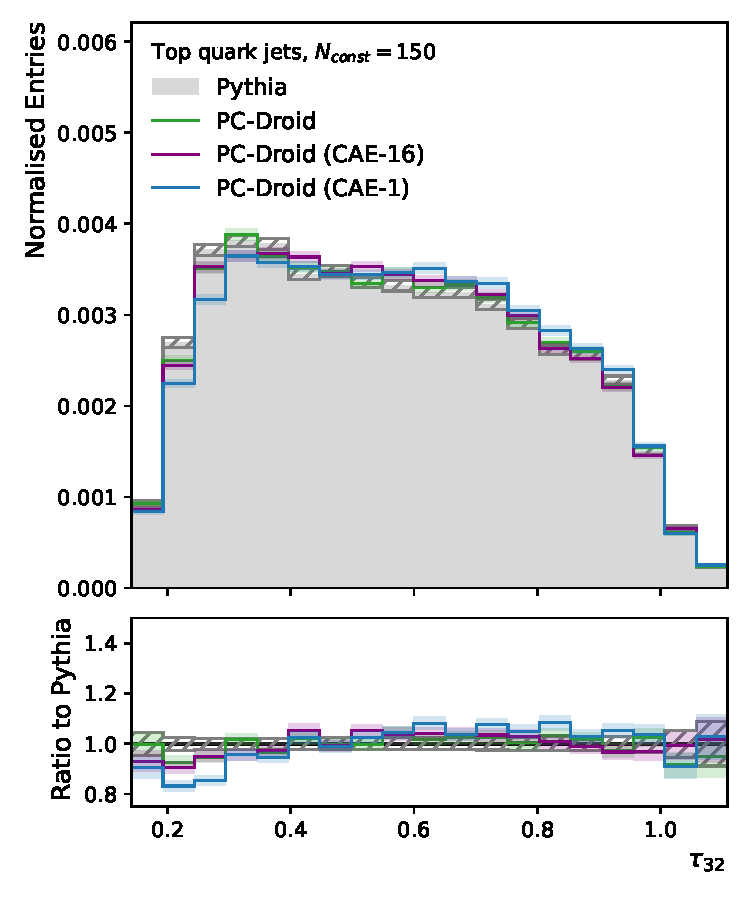
\includegraphics[width=0.33\textwidth]{Figures/jet_generation/droid/150/hlvs/t/100/tau_32.pdf}
    \caption{
        Comparison of the standard transformer based \pcdroid and the cross-attention encoder (CAE) variants using the generated mass and substructure marginals of top jets with up to 150 constituents.
    }
    \label{fig:hlvs-150-marginals}
\end{figure}

\begin{figure}[tb]
    \centering
    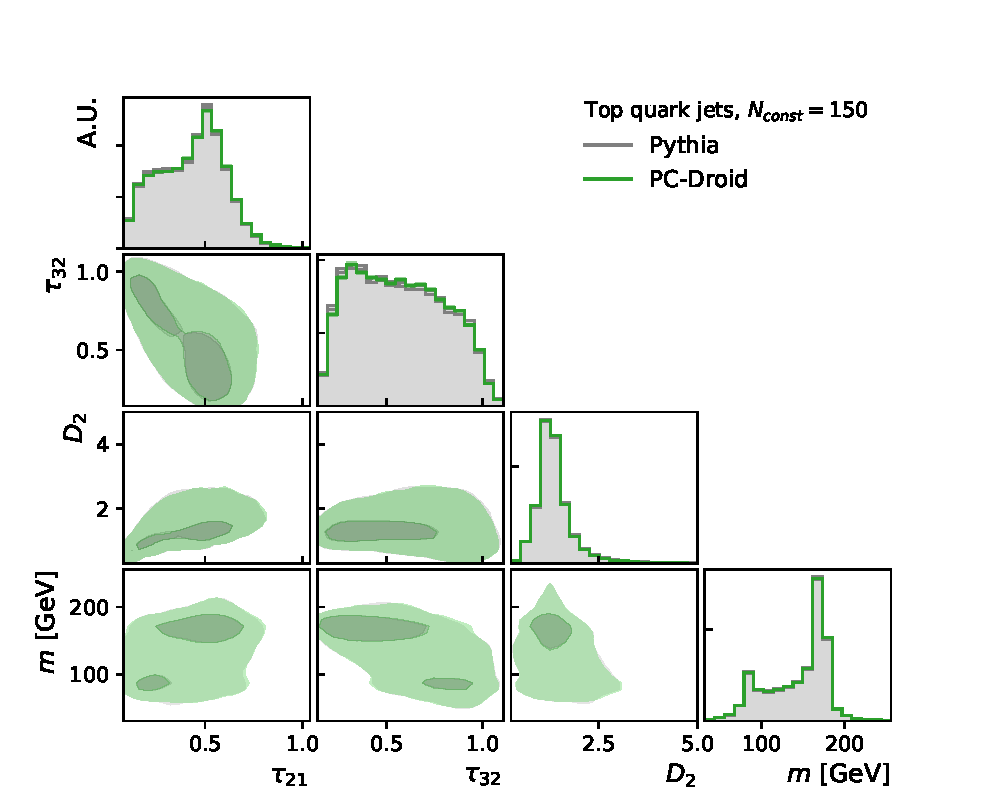
\includegraphics[width=0.49\textwidth]{Figures/jet_generation/droid/150/hlvs/t/100/hlv_corr_PC-Droid.pdf}
    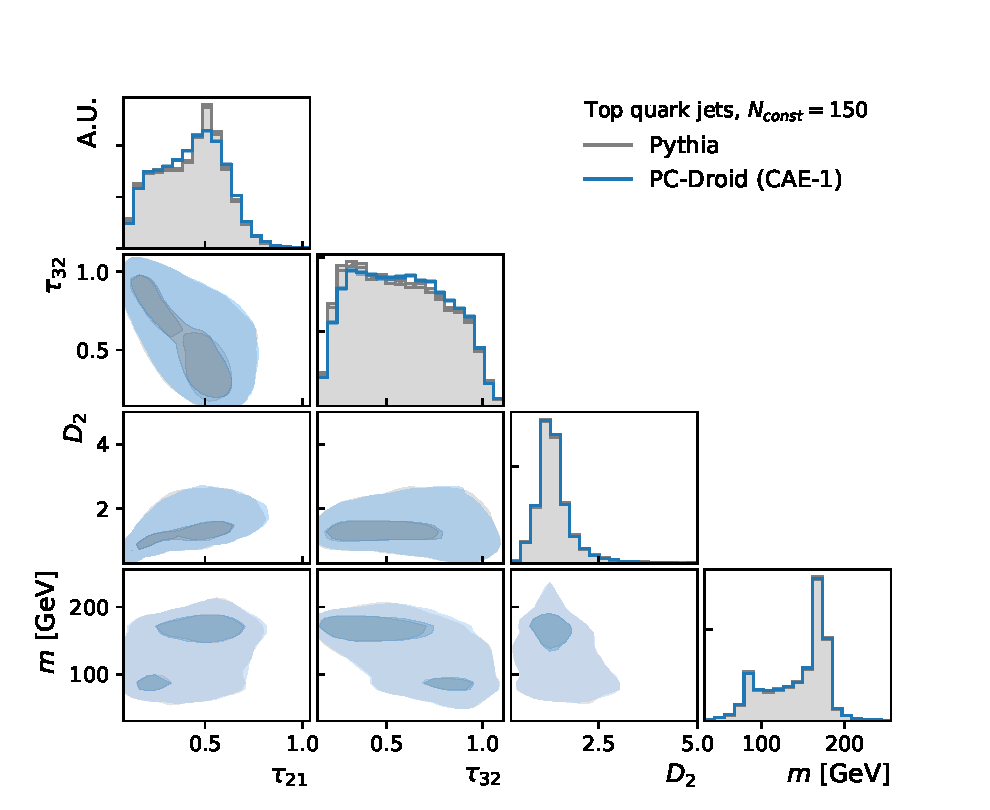
\includegraphics[width=0.49\textwidth]{Figures/jet_generation/droid/150/hlvs/t/100/hlv_corr_PC-DroidCAE1.pdf}
    \caption{
        Mass and substructure distributions of the generated top jets with up to 150 constituents.
        The diagonal consists of the marginals of the distributions and the off-diagonal elements contain the joint distributions.
    }
    \label{fig:hlvs-150}
\end{figure}

\begin{table}[tb]
    \centering
    \renewcommand{\arraystretch}{1.5}
    \caption{Comparison of generative models on top and gluon jets with up to 150 constituents. Lower is better. The FPND score is only defined for the first three classes and is sensitive only to the leading 30 constituents in \pt.}
    \label{tab:perf-150}
    \resizebox{\textwidth}{!}{%
        \begin{tabular}{llrrrrrrrc}
    \toprule
    Jet & Model             & NFE   & FPND            & $\mathrm{W_1^P}$ $(\times 10^{-4})$ & $\mathrm{W}_1^\mathrm{EFP}$ $(\times 10^{-6})$ & $\mathrm{W}_1^m$ $(\times 10^{-4})$ & $\mathrm{W}_1^{\tau_{21}}$ $(\times 10^{-3})$ & $\mathrm{W}_1^{\tau_{32}}$ $(\times 10^{-3})$ & $\mathrm{W}_1^{\Dtwo}$ $(\times 10^{-2})$ \\
    \midrule

    \multirow{10}{*}{Top}
        & \pythia           & $-$   & $0.01$          & $3.03 \pm 0.78$                     & $14.77 \pm 5.61$                               & $3.96 \pm 0.94$                     & $1.78 \pm 0.56$                               & $2.78 \pm 1.03$                               & $1.31 \pm 0.32$                           \\ \cline{2-10}
        & \pcdroid          & $100$ & $\mathbf{0.01}$ & $5.45 \pm 1.70$                     & $\mathbf{15.41 \pm 5.38}$                      & $\mathbf{3.60 \pm 1.20}$            & $\mathbf{2.87 \pm 1.20}$                      & $\mathbf{4.70 \pm 1.88}$                      & $\mathbf{1.15 \pm 0.30}$                  \\
        & \pcdroid (CAE-1)  & 100   & $0.06$          & $\mathbf{4.03 \pm 1.37}$            & $19.93 \pm 6.76$                               & $4.28 \pm 1.51$                     & $5.21 \pm 0.71$                               & $13.01 \pm 2.08$                              & $1.38 \pm 0.34$                           \\
        & \pcdroid (CAE-16) & 100   & $0.02$          & $5.40 \pm 1.43$                     & $17.17 \pm 5.85$                               & $4.63 \pm 1.28$                     & $3.22 \pm 0.61$                               & $5.94 \pm 1.55$                               & $1.31 \pm 0.28$                           \\
        & \pcdroid (CD1)    & $1$   & $0.13$          & $6.62 \pm 1.49$                     & $55.49 \pm 6.99$                               & $11.18 \pm 2.44$                    & $19.04 \pm 1.61$                              & $36.48 \pm 1.67$                              & $2.38 \pm 0.40$                           \\
        & \pcdroid (CD5)    & $5$   & $0.10$          & $6.78 \pm 1.76$                     & $54.25 \pm 5.27$                               & $9.24 \pm 1.53$                     & $7.53 \pm 0.79$                               & $22.98 \pm 1.58$                              & $1.31 \pm 0.30$                           \\
        & FPCD              & $512$ & $0.15$          & $4.36 \pm 1.28$                     & $26.11 \pm 6.30$                               & $6.44 \pm 2.57$                     & $6.30 \pm 0.81$                               & $9.91 \pm 1.39$                               & $1.47 \pm 0.36$                           \\
        & FPCD (PD1)        & $1$   & $0.53$          & $4.80 \pm 1.31$                     & $38.22 \pm 3.65$                               & $8.44 \pm 1.30$                     & $19.67 \pm 1.43$                              & $52.16 \pm 2.12$                              & $3.41 \pm 0.65$                           \\
        & EPiC-GAN          & $1$   & $0.95$          & $36.70 \pm 1.80$                    & $30.29 \pm 5.01$                               & $6.93 \pm 1.49$                     & $13.28 \pm 1.80$                              & $37.56 \pm 1.92$                              & $2.41 \pm 0.36$                           \\
    \midrule

    \multirow{10}{*}{Gluon}
        & \pythia           & $-$   & $0.01$          & $3.88 \pm 1.24$                     & $10.66 \pm 3.30$                               & $6.04 \pm 2.18$                     & $2.92 \pm 1.20$                               & $1.74 \pm 0.45$                               & $3.84 \pm 1.29$                           \\ \cline{2-10}
        & \pcdroid          & $100$ & $\mathbf{0.01}$ & $3.69 \pm 1.35$                     & $10.30 \pm 4.36$                               & $5.26 \pm 2.43$                     & $\mathbf{3.13 \pm 1.10}$                      & $\mathbf{2.24 \pm 0.93}$                      & $4.34 \pm 1.18$                           \\
        & \pcdroid (CAE-1)  & 100   & $\mathbf{0.01}$ & $\mathbf{3.38 \pm 1.10}$            & $11.84 \pm 4.15$                               & $\mathbf{4.62 \pm 1.29}$            & $4.07 \pm 1.30$                               & $2.41 \pm 0.75$                               & $\mathbf{3.27 \pm 1.39}$                  \\
        & \pcdroid (CAE-16) & 100   & $\mathbf{0.01}$ & $4.37 \pm 1.43$                     & $\mathbf{10.09 \pm 2.94}$                      & $5.04 \pm 1.77$                     & $3.22 \pm 1.06$                               & $\mathbf{2.24 \pm 0.72}$                      & $3.30 \pm 1.02$                           \\
        & \pcdroid (CD1)    & $1$   & $0.10$          & $6.54 \pm 1.81$                     & $21.55 \pm 6.13$                               & $5.55 \pm 2.76$                     & $15.33 \pm 2.58$                              & $10.73 \pm 0.80$                              & $4.52 \pm 1.12$                           \\
        & \pcdroid (CD5)    & $5$   & $0.06$          & $7.05 \pm 1.74$                     & $14.91 \pm 5.38$                               & $7.09 \pm 2.90$                     & $11.11 \pm 2.23$                              & $9.04 \pm 0.71$                               & $6.91 \pm 2.45$                           \\
        & FPCD              & $512$ & $0.03$          & $5.14 \pm 1.45$                     & $14.59 \pm 4.37$                               & $5.51 \pm 2.53$                     & $5.64 \pm 1.85$                               & $2.74 \pm 0.66$                               & $3.72 \pm 1.63$                           \\
        & FPCD (PD1)        & $1$   & $0.08$          & $5.53 \pm 1.24$                     & $18.83 \pm 5.71$                               & $6.83 \pm 1.61$                     & $19.36 \pm 2.45$                              & $10.97 \pm 1.03$                              & $7.83 \pm 1.60$                           \\
        & EPiC-GAN          & $1$   & $0.54$          & $32.22 \pm 1.83$                    & $12.72 \pm 4.14$                               & $5.00 \pm 1.47$                     & $15.49 \pm 2.14$                              & $13.32 \pm 1.08$                              & $4.03 \pm 1.15$                           \\
    \midrule

    \multirow{10}{*}{Quark}
        & \pythia           & $-$   & $0.01$          & $4.87 \pm 1.98$                     & $7.38 \pm 2.13$                                & $4.54 \pm 1.69$                     & $2.79 \pm 0.89$                               & $1.92 \pm 0.60$                               & $5.34 \pm 1.69$                           \\ \cline{2-10}
        & \pcdroid          & $100$ & $\mathbf{0.01}$ & $5.96 \pm 1.76$                     & $6.13 \pm 1.91$                                & $4.42 \pm 1.86$                     & $3.58 \pm 0.96$                               & $\mathbf{1.88 \pm 0.62}$                      & $\mathbf{6.42 \pm 2.68}$                  \\
        & \pcdroid (CAE-1)  & 100   & $\mathbf{0.01}$ & $\mathbf{4.55 \pm 1.03}$            & $6.04 \pm 1.86$                                & $\mathbf{3.88 \pm 1.53}$            & $4.02 \pm 1.35$                               & $2.07 \pm 0.51$                               & $6.45 \pm 1.35$                           \\
        & \pcdroid (CAE-16) & 100   & $0.02$          & $5.93 \pm 2.33$                     & $\mathbf{5.54 \pm 1.63}$                       & $4.82 \pm 1.56$                     & $\mathbf{3.52 \pm 0.91}$                      & $2.40 \pm 0.66$                               & $7.01 \pm 3.17$                           \\
        & \pcdroid (CD1)    & $1$   & $0.27$          & $7.74 \pm 2.21$                     & $9.90 \pm 2.69$                                & $6.50 \pm 1.87$                     & $13.56 \pm 1.89$                              & $9.22 \pm 0.60$                               & $24.58 \pm 2.17$                          \\
        & \pcdroid (CD5)    & $5$   & $0.15$          & $9.87 \pm 2.07$                     & $7.87 \pm 2.19$                                & $4.14 \pm 1.54$                     & $12.32 \pm 1.65$                              & $6.41 \pm 0.71$                               & $15.73 \pm 2.28$                          \\
        & FPCD              & $512$ & $0.03$          & $5.32 \pm 1.86$                     & $5.99 \pm 1.81$                                & $7.28 \pm 2.12$                     & $3.71 \pm 1.10$                               & $3.36 \pm 0.75$                               & $6.72 \pm 2.39$                           \\
        & FPCD (PD1)        & $1$   & $0.09$          & $6.39 \pm 1.94$                     & $7.24 \pm 2.14$                                & $7.43 \pm 2.84$                     & $17.58 \pm 1.75$                              & $9.40 \pm 0.98$                               & $18.71 \pm 2.52$                          \\
        & EPiC-GAN          & $1$   & $0.17$          & $39.69 \pm 2.67$                    & $8.19 \pm 3.06$                                & $5.25 \pm 1.78$                     & $13.00 \pm 1.85$                              & $10.35 \pm 0.89$                              & $26.65 \pm 3.21$                          \\
    \midrule

    \multirow{9}{*}{W Boson}
        & \pythia           & $-$   & $-$             & $3.86 \pm 1.16$                     & $1.87 \pm 0.51$                                & $1.73 \pm 0.47$                     & $2.79 \pm 0.83$                               & $3.19 \pm 1.31$                               & $2.95 \pm 1.21$                           \\ \cline{2-10}
        & \pcdroid          & $100$ & $-$             & $\mathbf{3.32 \pm 0.98}$            & $\mathbf{1.49 \pm 0.38}$                       & $\mathbf{1.72 \pm 0.75}$            & $3.33 \pm 1.12$                               & $\mathbf{2.14 \pm 0.61}$                      & $\mathbf{2.73 \pm 0.99}$                  \\
        & \pcdroid (CAE-1)  & 100   & $-$             & $3.79 \pm 1.12$                     & $1.58 \pm 0.48$                                & $2.18 \pm 0.51$                     & $3.00 \pm 1.08$                               & $3.59 \pm 1.27$                               & $2.75 \pm 0.78$                           \\
        & \pcdroid (CAE-16) & 100   & $-$             & $3.93 \pm 1.03$                     & $1.82 \pm 0.49$                                & $2.04 \pm 0.56$                     & $\mathbf{2.81 \pm 0.83}$                      & $2.62 \pm 1.09$                               & $3.21 \pm 1.45$                           \\
        & \pcdroid (CD1)    & $1$   & $-$             & $5.06 \pm 1.16$                     & $6.47 \pm 0.89$                                & $12.80 \pm 0.93$                    & $26.98 \pm 1.57$                              & $10.64 \pm 0.73$                              & $6.42 \pm 0.74$                           \\
        & \pcdroid (CD5)    & $5$   & $-$             & $6.25 \pm 1.07$                     & $4.40 \pm 0.62$                                & $8.28 \pm 0.43$                     & $8.07 \pm 1.48$                               & $13.30 \pm 1.44$                              & $3.94 \pm 1.20$                           \\
        & FPCD              & $512$ & $-$             & $3.53 \pm 1.06$                     & $2.02 \pm 0.58$                                & $2.97 \pm 0.41$                     & $2.86 \pm 0.91$                               & $3.91 \pm 0.84$                               & $2.92 \pm 0.86$                           \\
        & FPCD (PD1)        & $1$   & $-$             & $4.32 \pm 1.40$                     & $4.00 \pm 0.57$                                & $9.07 \pm 0.51$                     & $20.78 \pm 1.48$                              & $7.90 \pm 0.45$                               & $7.31 \pm 1.22$                           \\
    \midrule

    \multirow{9}{*}{Z Boson}
        & \pythia           & $-$   & $-$             & $4.12 \pm 1.57$                     & $2.10 \pm 0.54$                                & $2.19 \pm 0.77$                     & $3.10 \pm 1.49$                               & $2.00 \pm 0.59$                               & $3.42 \pm 0.94$                           \\ \cline{2-10}
        & \pcdroid          & $100$ & $-$             & $3.90 \pm 1.32$                     & $\mathbf{2.01 \pm 0.67}$                       & $1.95 \pm 0.52$                     & $\mathbf{2.71 \pm 0.99}$                      & $\mathbf{2.22 \pm 0.62}$                      & $3.22 \pm 0.95$                           \\
        & \pcdroid (CAE-1)  & 100   & $-$             & $\mathbf{3.65 \pm 1.14}$            & $2.04 \pm 0.68$                                & $2.24 \pm 0.58$                     & $3.43 \pm 1.02$                               & $4.16 \pm 1.13$                               & $\mathbf{2.43 \pm 0.58}$                  \\
        & \pcdroid (CAE-16) & 100   & $-$             & $3.87 \pm 1.15$                     & $2.19 \pm 0.53$                                & $\mathbf{1.90 \pm 0.73}$            & $3.28 \pm 1.18$                               & $2.58 \pm 1.04$                               & $3.08 \pm 0.92$                           \\
        & \pcdroid (CD1)    & $1$   & $-$             & $5.04 \pm 0.94$                     & $6.57 \pm 0.73$                                & $12.20 \pm 0.53$                    & $22.78 \pm 2.07$                              & $9.32 \pm 0.67$                               & $6.12 \pm 1.09$                           \\
        & \pcdroid (CD5)    & $5$   & $-$             & $5.41 \pm 1.21$                     & $6.16 \pm 0.74$                                & $7.99 \pm 0.45$                     & $6.39 \pm 1.28$                               & $15.49 \pm 1.23$                              & $3.40 \pm 0.88$                           \\
        & FPCD              & $512$ & $-$             & $4.66 \pm 1.35$                     & $2.59 \pm 0.61$                                & $2.97 \pm 0.53$                     & $3.90 \pm 1.35$                               & $4.26 \pm 1.14$                               & $3.05 \pm 0.73$                           \\
        & FPCD (PD1)        & $1$   & $-$             & $4.72 \pm 1.26$                     & $5.91 \pm 0.75$                                & $9.63 \pm 0.93$                     & $23.70 \pm 1.76$                              & $8.52 \pm 1.08$                               & $6.55 \pm 1.04$                           \\
    \bottomrule
\end{tabular}

    }
\end{table}

\FloatBarrier

\subsubsection{Conditional Adherence}

As \pcdroid is a conditional generative model, it was crucial to determine if the model generates jets with kinematics consistent with the conditioning values.
To test this, we examine the difference between the generated point cloud kinematics and the target conditions for mass and \pt, as shown in Figure \ref{fig:obedience}.

The exact jet kinematics from the simulation are used for the \textit{conditional kinematics}, while the \textit{point cloud kinematics} are recalculated from the preprocessed jet constituents.
These different approaches result in minor discrepancies between the variables, even for the \pythia dataset.
The original jets may have had more than 150 constituents when the kinematics were calculated, causing a negative shift in mass and \pt.

In the mass plot in Figure \ref{fig:obedience}, \pcdroid displays a nearly identical spread to \pythia.
For \pt, there is slightly more variation with higher residual magnitudes, but \pcdroid remains within $0.4\%$ of the target.

\begin{figure}[htpb]
    \centering
    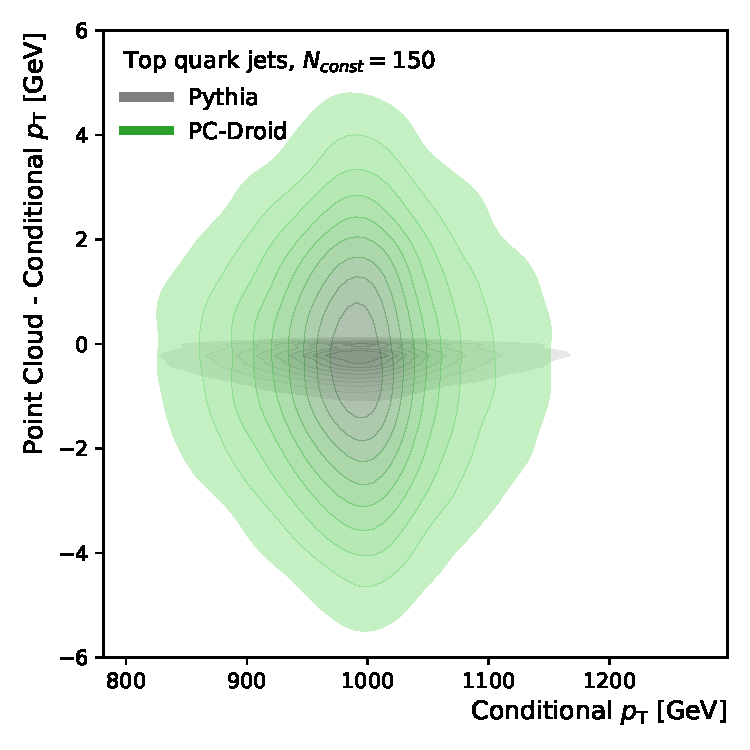
\includegraphics[width=0.32\textwidth]{Figures/jet_generation/droid/150/obedience/t/100/t_pt_PC-Droid_resid.pdf}
    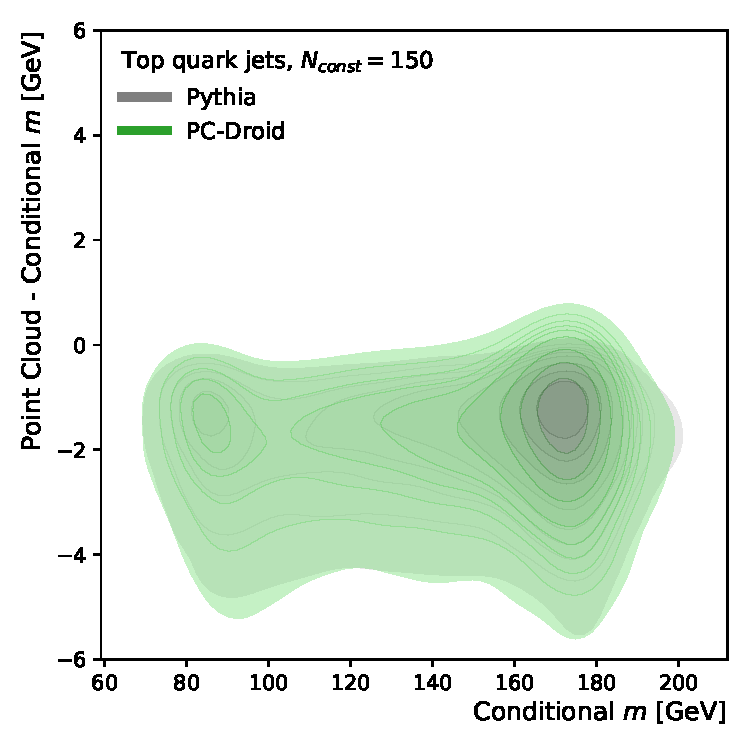
\includegraphics[width=0.32\textwidth]{Figures/jet_generation/droid/150/obedience/t/100/t_mass_PC-Droid_resid.pdf}
    \caption{The correlation between the conditional and point cloud kinematics on top jets with up to 150 constituents. The $y$-axis, shows the difference between the two variables.}
    \label{fig:obedience}
\end{figure}

\subsubsection{Consistency Distillation}

Diffusion models inherently present a trade-off between the number of iterations during generation and the quality of the final sample.
Consistency models add another dimension to this trade-off by enabling the production of reasonable samples in as few as one iteration step.
Consistency models significantly outperform diffusion models when constrained to minimal steps.

To enhance generation speed and examine its impact on performance, we train a consistency model using \pcdroid as the teacher.
We adopt the same training configuration as the original paper by \textcite{ConsistencyModels} with one modification: instead of employing the Heun integration solver to select adjacent points of the ODE, we find that DPM2 yields improved performance.
During generation, we achieve reasonable performance with just a single network pass and observe that performance plateaus after five steps.

\Cref{fig:cd-150} compares the substructure variables for jets produced using the CD model with one-step (CD1) and multi-step (CD5) generation.
The top jet subjettiness ratios continue to be the most challenging to reproduce, but the one-step consistency model also demonstrates a general broadening in the mass distribution.

\begin{figure}[htpb]
    \centering
    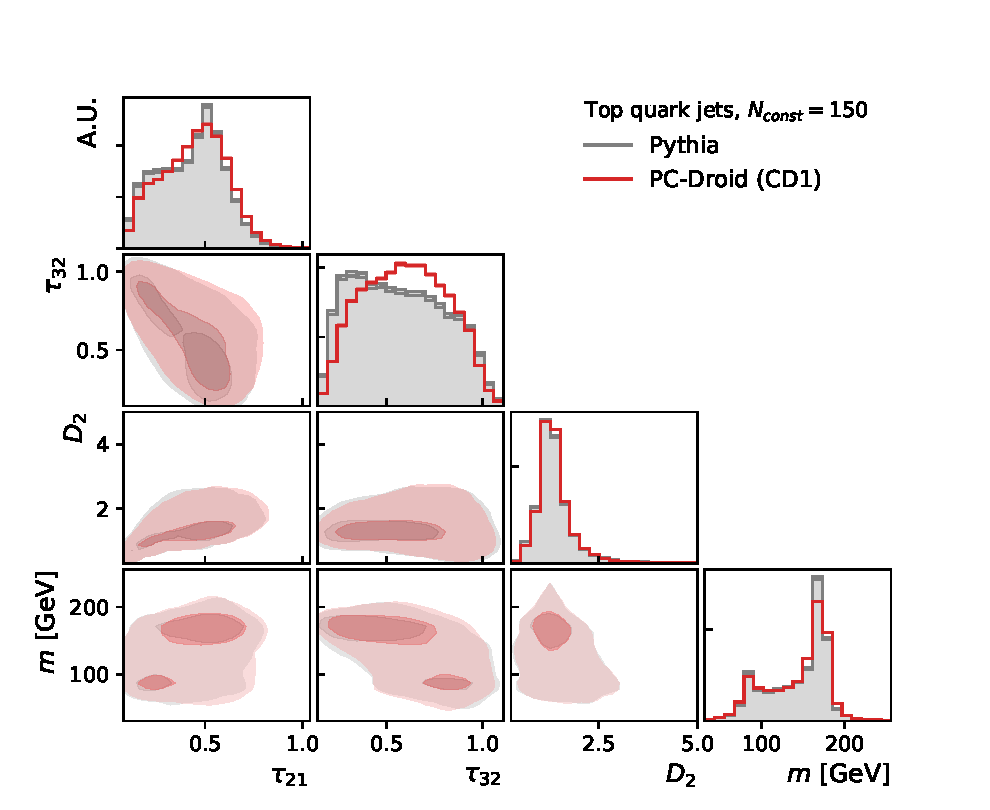
\includegraphics[width=0.49\textwidth]{Figures/jet_generation/droid/150/hlvs/t/100/hlv_corr_PC-DroidCD1.pdf}
    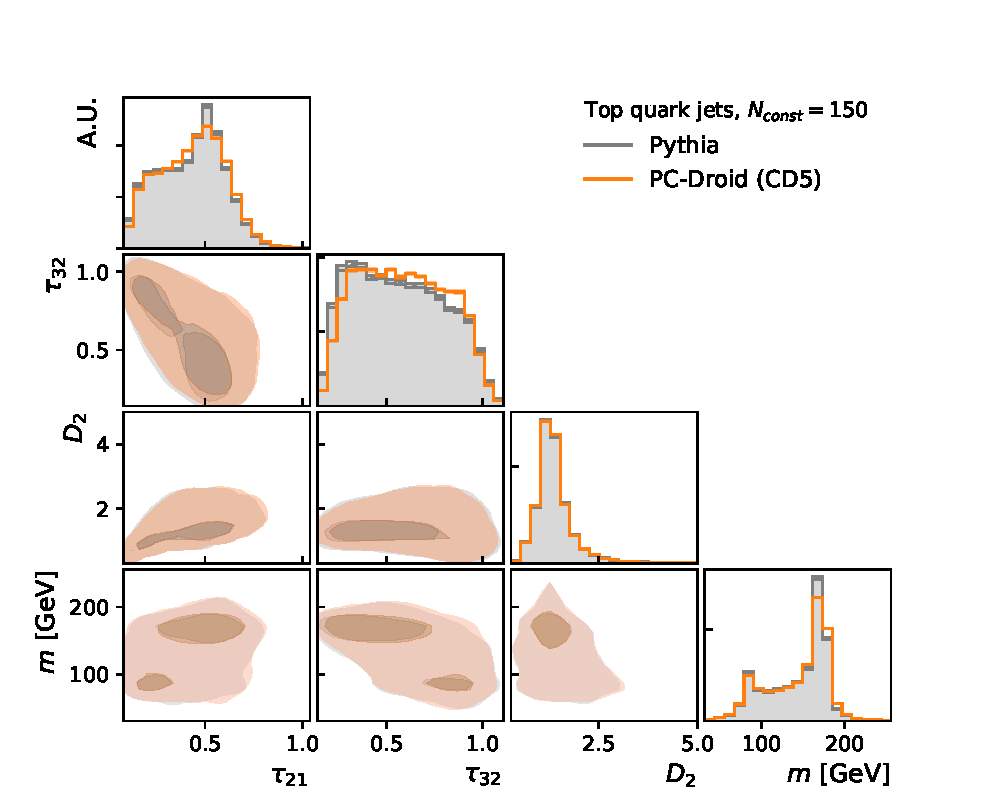
\includegraphics[width=0.49\textwidth]{Figures/jet_generation/droid/150/hlvs/t/100/hlv_corr_PC-DroidCD5.pdf}
    \caption{
        Mass and substructure distributions of the generated top jets with up to 150 constituents using the CD models.
        The diagonal consists of the marginals and the off-diagonal elements contain the joint distributions.
    }
    \label{fig:cd-150}
\end{figure}

\subsubsection{Modelling The Conditional Variables}

Utilizing normalizing flows, we have the flexibility to sample either the complete set of jet kinematics along with $N_{const}$ (Flow-$\p$) or just $N_{const}$ (Flow-$N$), both conditional on PID.
It is crucial to emphasize that these flows are trained independently of \pcdroid, as this constitutes an entirely orthogonal task.
The performance of Flow-$\p$ is showcased in \Cref{fig:unconditional-flows}, illustrating that the marginals and correlations of the conditioning variables are accurately modelled.

We evaluate the conditional and unconditional models using the full array of metrics in \Cref{tab:perf-150-unconditional}.
Here, \pcdroid denotes the conditional model, where $N_{const}$ and the jet kinematics are derived from the test set.
The other two rows represent scenarios where either flow is used to initially sample these variables before passing them to the diffusion model.
Notably, there is minimal difference in performance when shifting to unconditional generation, and \pcjedi continues to outperform other methods significantly.

\begin{figure}[b!]
    \centering
    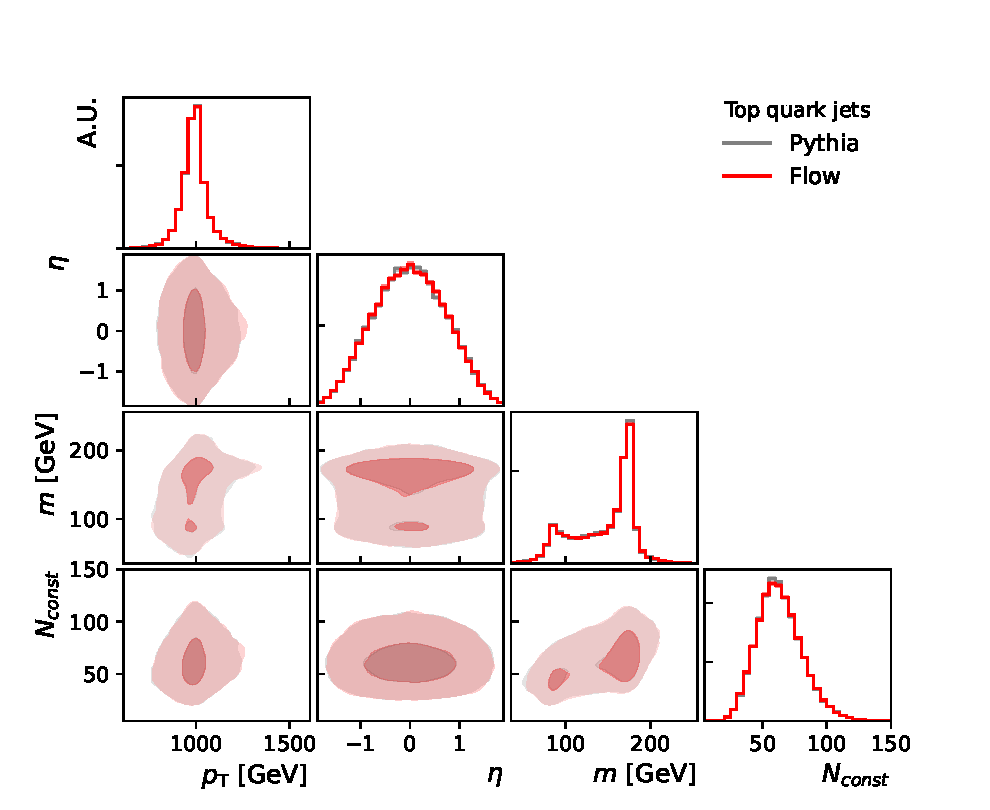
\includegraphics[width=0.49\linewidth]{Figures/jet_generation/droid/150/flow_quality_t.pdf}
    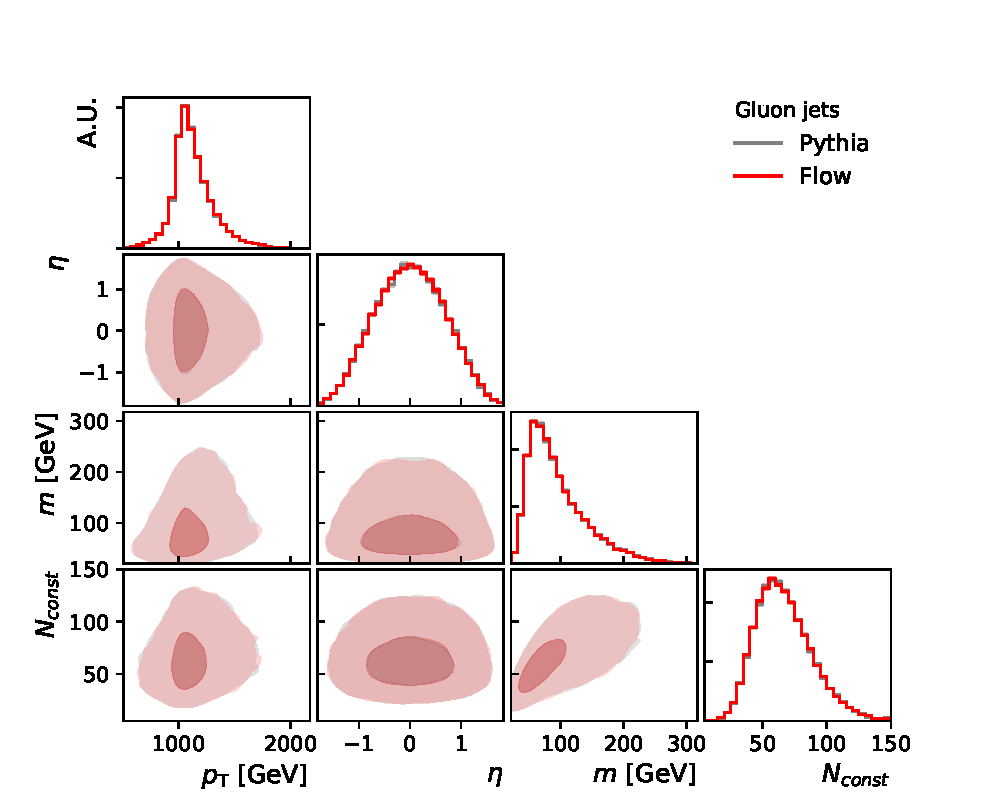
\includegraphics[width=0.49\linewidth]{Figures/jet_generation/droid/150/flow_quality_g.pdf}
    \caption{Marginals of the conditioning variables generated with Flow-$\p$ compared to \pythia for top and gluon jets with up to 150 constituents.
    }
    \label{fig:unconditional-flows}
\end{figure}

\begin{table}[tp]
    \centering
    \renewcommand{\arraystretch}{1.5}
    \caption{Comparison of conditional and unconditional models on jets with up to 150 constituents. The FPND score is only defined for the first three classes and is sensitive only to the leading 30 constituents in \pt.
    }
    \label{tab:perf-150-unconditional}
    \resizebox{\textwidth}{!}{%
        \begin{tabular}{llrrrrrrr}
    \toprule
    Jet & Model                & FPND            & $\mathrm{W_1^P}$ $(\times 10^{-4})$ & $\mathrm{W}_1^\mathrm{EFP}$ $(\times 10^{-6})$ & $\mathrm{W}_1^m$ $(\times 10^{-4})$ & $\mathrm{W}_1^{\tau_{21}}$ $(\times 10^{-3})$ & $\mathrm{W}_1^{\tau_{32}}$ $(\times 10^{-3})$ & $\mathrm{W}_1^{\Dtwo}$ $(\times 10^{-2})$ \\
    \midrule

    \multirow{4}{*}{Top}
        & \pythia              & $0.01$          & $3.03 \pm 0.78$                     & $14.77 \pm 5.61$                               & $3.96 \pm 0.94$                     & $1.78 \pm 0.56$                               & $2.78 \pm 1.03$                               & $1.31 \pm 0.32$                           \\ \cline{2-9}
        & \pcdroid             & $\mathbf{0.01}$ & $5.45 \pm 1.70$                     & $15.41 \pm 5.38$                               & $\mathbf{3.60 \pm 1.20}$            & $2.87 \pm 1.20$                               & $4.70 \pm 1.88$                               & $\mathbf{1.15 \pm 0.30}$                  \\
        & \pcdroid (Flow-$\p$) & $0.02$          & $4.95 \pm 1.34$                     & $17.97 \pm 4.44$                               & $4.84 \pm 1.18$                     & $3.40 \pm 1.29$                               & $5.35 \pm 1.33$                               & $1.23 \pm 0.36$                           \\
        & \pcdroid (Flow-$N$)  & $\mathbf{0.01}$ & $\mathbf{4.89 \pm 1.47}$            & $\mathbf{14.14 \pm 3.93}$                      & $3.91 \pm 1.35$                     & $3.39 \pm 1.28$                               & $5.28 \pm 1.33$                               & $1.38 \pm 0.27$                           \\
    \midrule

    \multirow{4}{*}{Gluon}
        & \pythia              & $0.01$          & $3.88 \pm 1.24$                     & $10.66 \pm 3.30$                               & $6.04 \pm 2.18$                     & $2.92 \pm 1.20$                               & $1.74 \pm 0.45$                               & $3.84 \pm 1.29$                           \\ \cline{2-9}
        & \pcdroid             & $\mathbf{0.01}$ & $3.69 \pm 1.35$                     & $10.30 \pm 4.36$                               & $5.26 \pm 2.43$                     & $3.13 \pm 1.10$                               & $2.24 \pm 0.93$                               & $4.34 \pm 1.18$                           \\
        & \pcdroid (Flow-$\p$) & $\mathbf{0.01}$ & $\mathbf{3.63 \pm 1.56}$            & $10.63 \pm 2.07$                               & $6.10 \pm 3.02$                     & $3.43 \pm 1.19$                               & $2.24 \pm 0.91$                               & $4.50 \pm 1.82$                           \\
        & \pcdroid (Flow-$N$)  & $0.02$          & $4.01 \pm 1.22$                     & $\mathbf{9.74 \pm 2.53}$                       & $\mathbf{4.90 \pm 1.54}$            & $3.40 \pm 1.21$                               & $\mathbf{2.20 \pm 0.90}$                      & $\mathbf{3.13 \pm 0.83}$                  \\
    \midrule

    \multirow{4}{*}{Quark}
        & \pythia              & $0.01$          & $4.87 \pm 1.98$                     & $7.38 \pm 2.13$                                & $4.54 \pm 1.69$                     & $2.79 \pm 0.89$                               & $1.92 \pm 0.60$                               & $5.34 \pm 1.69$                           \\ \cline{2-9}
        & \pcdroid             & $\mathbf{0.01}$ & $5.96 \pm 1.76$                     & $\mathbf{6.13 \pm 1.91}$                       & $4.42 \pm 1.86$                     & $3.58 \pm 0.96$                               & $1.88 \pm 0.62$                               & $6.42 \pm 2.68$                           \\
        & \pcdroid (Flow-$\p$) & $\mathbf{0.01}$ & $7.18 \pm 2.33$                     & $6.46 \pm 1.42$                                & $4.83 \pm 1.41$                     & $2.95 \pm 1.04$                               & $2.26 \pm 0.79$                               & $\mathbf{5.70 \pm 2.00}$                  \\
        & \pcdroid (Flow-$N$)  & $\mathbf{0.01}$ & $\mathbf{5.52 \pm 1.86}$            & $6.40 \pm 1.82$                                & $\mathbf{4.19 \pm 1.07}$            & $\mathbf{2.92 \pm 1.05}$                      & $2.26 \pm 0.78$                               & $6.86 \pm 2.07$                           \\
    \midrule

    \multirow{4}{*}{W Boson}
        & \pythia              & $-$             & $3.86 \pm 1.16$                     & $1.87 \pm 0.51$                                & $1.73 \pm 0.47$                     & $2.79 \pm 0.83$                               & $3.19 \pm 1.31$                               & $2.95 \pm 1.21$                           \\ \cline{2-9}
        & \pcdroid             & $-$             & $\mathbf{3.32 \pm 0.98}$            & $\mathbf{1.49 \pm 0.38}$                       & $1.72 \pm 0.75$                     & $3.33 \pm 1.12$                               & $2.14 \pm 0.61$                               & $\mathbf{2.73 \pm 0.99}$                  \\
        & \pcdroid (Flow-$\p$) & $-$             & $3.77 \pm 1.08$                     & $2.07 \pm 0.50$                                & $2.27 \pm 0.58$                     & $3.02 \pm 1.02$                               & $3.27 \pm 1.04$                               & $2.81 \pm 0.93$                           \\
        & \pcdroid (Flow-$N$)  & $-$             & $3.62 \pm 0.98$                     & $1.82 \pm 0.44$                                & $\mathbf{1.70 \pm 0.58}$            & $3.08 \pm 1.01$                               & $3.31 \pm 1.06$                               & $2.82 \pm 0.89$                           \\
    \midrule


    \multirow{4}{*}{Z Boson}
        & \pythia              & $-$             & $4.12 \pm 1.57$                     & $2.10 \pm 0.54$                                & $2.19 \pm 0.77$                     & $3.10 \pm 1.49$                               & $2.00 \pm 0.59$                               & $3.42 \pm 0.94$                           \\ \cline{2-9}
        & \pcdroid             & $-$             & $3.90 \pm 1.32$                     & $2.01 \pm 0.67$                                & $1.95 \pm 0.52$                     & $2.71 \pm 0.99$                               & $2.22 \pm 0.62$                               & $3.22 \pm 0.95$                           \\
        & \pcdroid (Flow-$\p$) & $-$             & $\mathbf{3.62 \pm 1.07}$            & $1.86 \pm 0.39$                                & $1.95 \pm 0.69$                     & $3.03 \pm 1.05$                               & $2.34 \pm 0.67$                               & $2.72 \pm 0.71$                           \\
        & \pcdroid (Flow-$N$)  & $-$             & $4.46 \pm 1.48$                     & $\mathbf{1.81 \pm 0.51}$                       & $\mathbf{1.70 \pm 0.66}$            & $3.01 \pm 1.06$                               & $2.31 \pm 0.67$                               & $\mathbf{2.56 \pm 0.80}$                  \\
    \bottomrule
\end{tabular}

    }
\end{table}

\FloatBarrier

\subsubsection{Timing Studies}

We examined the trade-off between quality and generation time across all models.
\Cref{fig:timing} illustrates three key metrics for all models as a function of the generation time required to produce top jets with 150 constituents on identical hardware.
All times are derived from the average of ten runs, each generating a batch of 512 jets using an NVIDIA GeForce 3080.
All scores are benchmarked against the ideal performance, as defined by the \pythia datasets.

Our fastest model (CD1) requires three times the generation time of EPiC-GAN but induces a slight shift in the jet mass but improves the FPND score considerably.
It is nearly 30\% faster than one step FPCD~(PD1) and shows markedly improved performance, especially in FPND.
The $\tau_{32}$ scores of these models are comparable.
CD5, although five times slower than the one-shot generation, improves all metrics across the board.
CAE-1 further enhances all metrics, particularly $\mathrm{W}_1^m$.
By increasing the number of global tokens to 16, we observe a 50\% increase in generation time but a significant improvement in both FPND and $\mathrm{W}1^{\tau{32}}$.
The full \pcdroid model, while approximately 250 times slower than EPiC-GAN, achieves nearly ideal performance in all metrics except $\mathrm{W}1^{\tau{32}}$, and is still around 4 times faster than the \pythia simulation.

\begin{figure}[htbp]
    \centering
    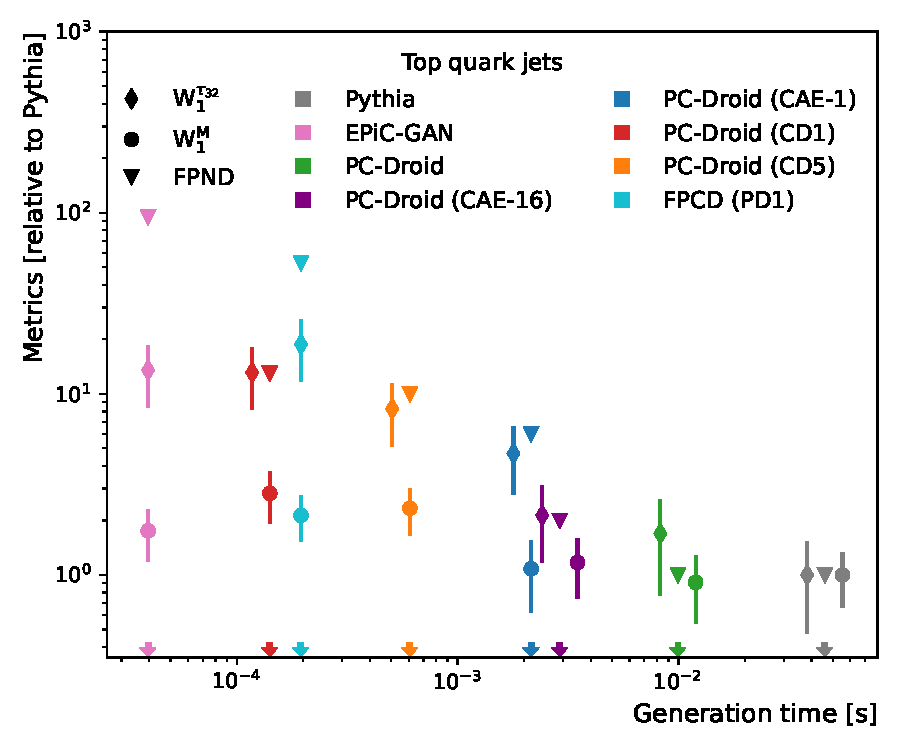
\includegraphics[width=0.5\textwidth]{Figures/jet_generation/droid/150/metrics_vs_times/t/t_metrics_vs_times.pdf}
    \caption{Performance as a ratio to \pythia as a function of the required generation time for a top jet with up to 150 constituents. The time for \pythia is taken from Ref.~\cite{MPGAN}.}
    \label{fig:timing}
\end{figure}

\subsection{Diffusion with EPiC Layers}

We collaborated with the research group responsible for the EPiC-GAN model, integrating our diffusion model with their EPiC layers~\cite{EpicJedi}.
In this study, we also experimented with using the CFM framework to describe the diffusion process, which was significantly more efficient than the SM-TI framework employed in \pcjedi.
This research was conducted concurrently with the development of the \pcdroid and thus only compared to the \pcjedi model.

Utilizing these layers, we achieved approximately a seven-fold increase in generation speed over the transformer.
The resulting performance and generation time was comparable to the CAE-1 model from \pcdroid.
One again, the subjettiness ratios remained particularly challenging to model for top jets, as illustrated in \Cref{fig:epic-diffusion}.

An area yet to be explored is the comparison between the CFM and EDM frameworks for this specific task.
While generative models for text-to-image generation have transitioned from EDM to CFM over the past year~\cite{SD3,flux2024github}, it remains uncertain if this trend applies to jet generation.

\begin{figure}[tb]
    \centering
    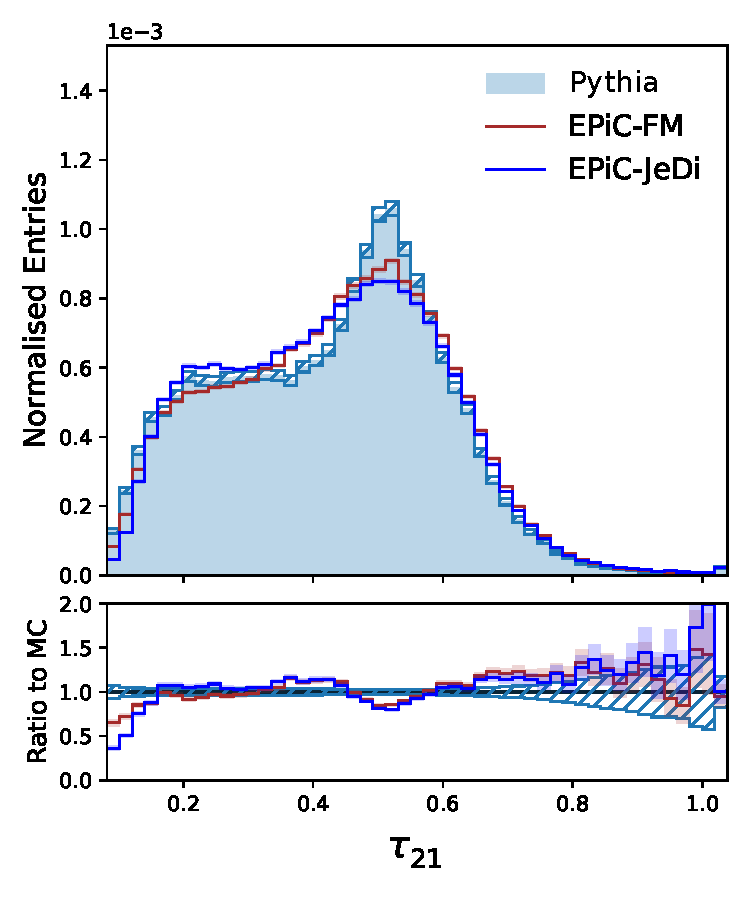
\includegraphics[width=0.33\textwidth]{Figures/jet_generation/t_tau21.pdf}
    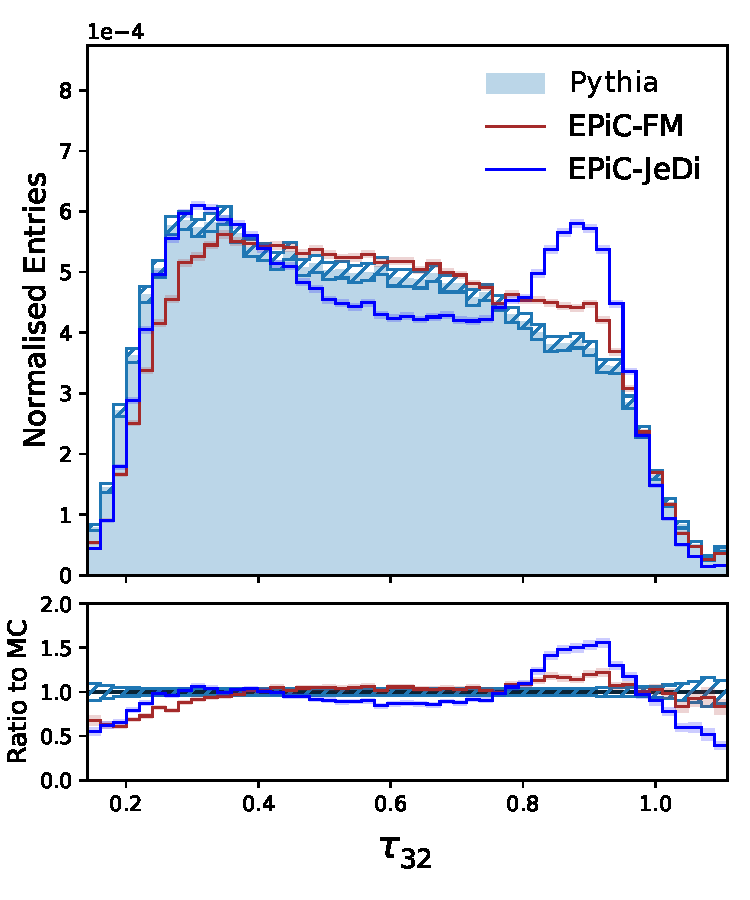
\includegraphics[width=0.33\textwidth]{Figures/jet_generation/t_tau32.pdf}
    \caption{
        Comparison between generative models using EPiC layers using the diffusion framework from \pcjedi verses the CFM framework.
    }
    \label{fig:epic-diffusion}
\end{figure}

\subsection{Conclusion}

Generative models employing diffusion processes present numerous points along the continuum between generation time and output quality.
In this research, we have expanded the scope by introducing new components to this trade-off.
We switched to the much more theoretically motivated EDM framework, which instantly yielded superior results compared to \pcjedi.
We have incorporated additional integration solvers to further enhance generation and consistency distillation, producing derived models with ODEs with straighter paths, which can be calculated in fewer integration steps.
We have also developed the CAE Block, which can scale to generate sets with higher multiplicities due to reduced computational overhead.

Our top-performing model approaches saturation across nearly all evaluative metrics for various jet types.
The sole exception remains the complex subjettiness ratios within top jets, which encompass both three- and two-pronged jets.

Our framework represents a significant advancement in high-quality jet generation.
It is now primed for applications in forward simulation and as a template construction tool for anomaly detection.

\section{Full Forward Simulation}

This enables physicists to quickly generate large amounts of high-fidelity simulated data, essential for designing experiments, optimizing detector configurations, and interpreting results from particle collisions. Ultimately, generative modeling enhances our ability to explore the fundamental laws of nature at unprecedented scales and speeds.



To test the model in a forward simulation setting we used the \pcdroid framework in a set-to-set generation task.
This section is a brief summary of the work presented in~\textcite{PIPPIN}.
This method, called PIPPIN conditionally generated the full collection of physics objects at reco-level (post detector simulation and reconstruction) from the set of particles at truth-level (before any showering or hadronization).

For this task we used a custom dataset of \ttbar events matching the setup in \Cref{sec:data} except without any constraints on the decay channels of the top quarks of the W bosons.

To address the challenge of multiplicity variations between the parton and reconstructed object spaces we used a combination of transformers, diffusion models and normalizing flows.
In the PIPPIN model, the set of truth-level particles is first passed through a transformer encoder to produce a set of embedded tokens.
These are used in two separate models.
The first is the multiplicity predictor.
One of the main challenges in this set-to-set task was predicting how the cardinality of the reco-level set.
In addition, this cardinality could be defined for each object type (jets, leptons, photons).
We defined as a single vector $N_x$ which contained the number of each object type.
This is a normalising flow which is trained to predict the number of reconstructed leptons, photons, and jets that the parton-set will produce.
The flow models all of these multiplicities together using a single vector $N_x$ conditioned on the embedded parton tokens.
This vector had to undergo dequantization when in forward mode and rounding when in reverse mode to model the discrete nature of the multiplicity.
The second model is the denoising diffusion model.
This model is trained to denoise the set of reco-level objects and their attributes and is constructed similarly to \pcdroid.
The main difference is that since it is conditioned on the output of the parton transformer, it is built as a transformer encoder, with additional cross-attention layers.
A diagram of the information flow used during training is shown in \Cref{fig:pippin}.
The two losses, from the multiplicity predictor and the denoising diffusion model, are combined to train the full PIPPIN model.

\begin{figure}[tb]
    \centering
    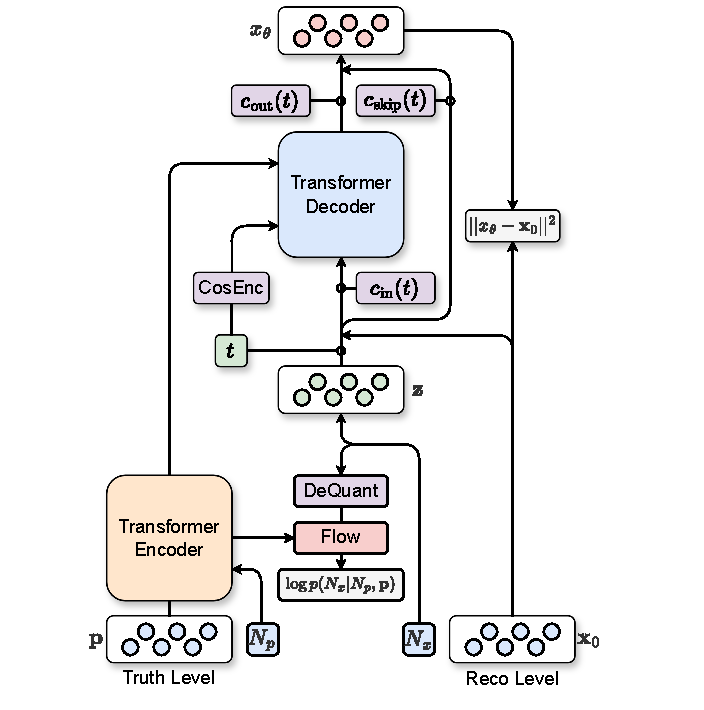
\includegraphics[width=0.70\textwidth]{Figures/jet_generation/PIPPIN.pdf}
    \caption{
        The PIPPIN model architecture which conditionally generates the full set of reconstructed (reco) physics objects from the set of truth-level objects.
    }
    \label{fig:pippin}
\end{figure}

The results from this model were highly promising.
The multiplicity predictor was able to match the marginals of the true multiplicities to within a few percent, as well as provide unbiased predictions as, shown in \Cref{fig:pippin_n}.
The denoising diffusion model was able to generate reco-level objects with high fidelity to the true objects, as shown in \Cref{fig:pippin_jet}.
Including for performing combined reconstruction to identify top quarks and W bosons, as shown in \Cref{fig:pippin_mass}.

We compared with two other deep generative models for this type of task, OTUS~\cite{OTUS} and Turbo-Sim~\cite{TurboSim}.
The main metrics were the Kolmogorov-Smirnov distances between the original MC reco-level distributions and the output of the different models.
As shown in \Cref{tab:pippin}, the PIPPIN model outperformed both OTUS and Turbo-Sim in all metrics.

\begin{figure}[htb]
    \centering
    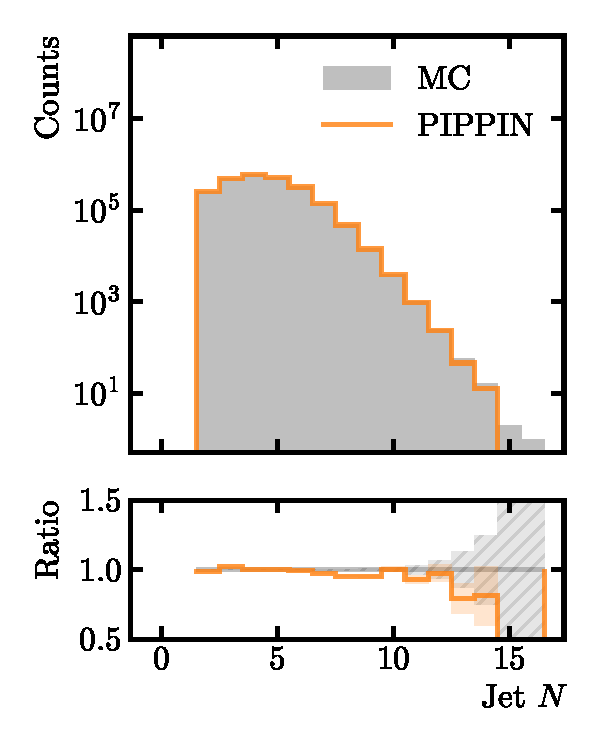
\includegraphics[width=0.32\textwidth]{Figures/jet_generation/pippin/marginals/marginal_jet_n.pdf}
    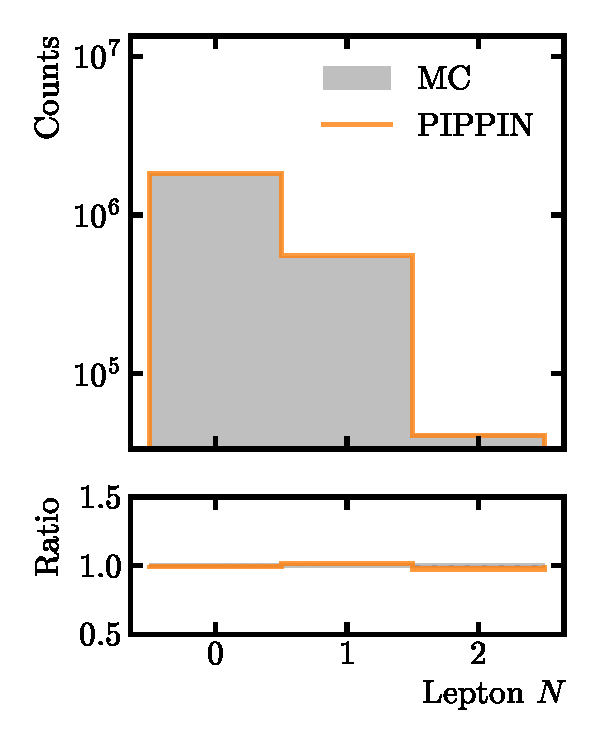
\includegraphics[width=0.32\textwidth]{Figures/jet_generation/pippin/marginals/marginal_lep_n.pdf} \\
    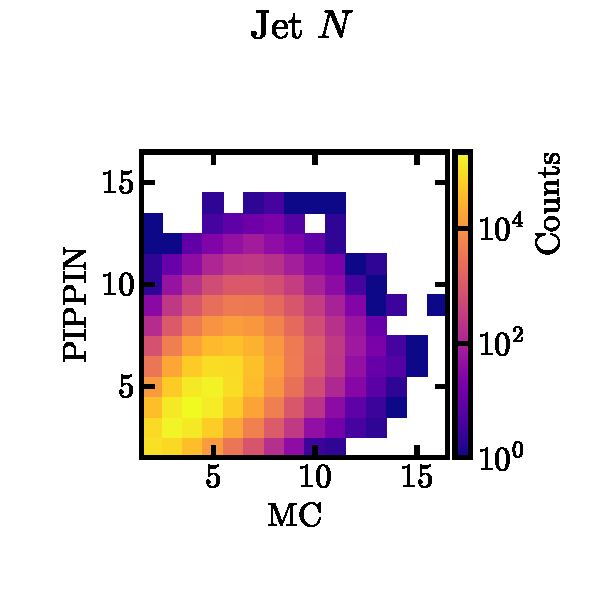
\includegraphics[clip, trim=0cm 0cm 0cm 2.5cm, width=0.32\textwidth]{Figures/jet_generation/pippin/marginals_2D/marginal2D_jet_n.pdf}
    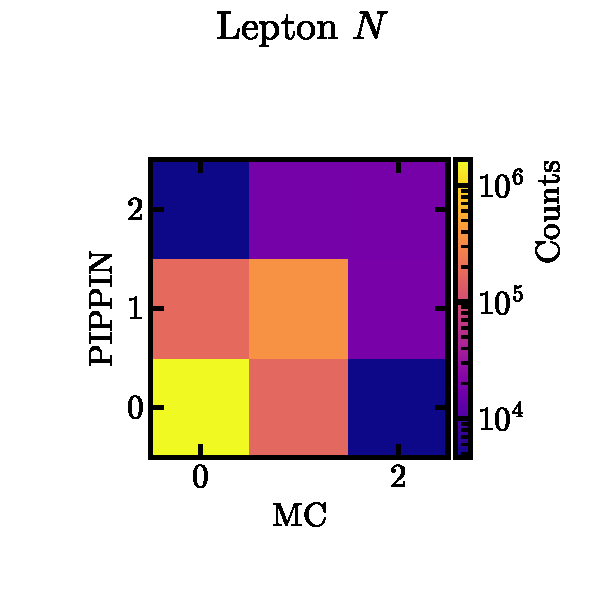
\includegraphics[clip, trim=0cm 0cm 0cm 2.5cm, width=0.32\textwidth]{Figures/jet_generation/pippin/marginals_2D/marginal2D_lep_n.pdf}
    \caption{
        The marginal and conditional distributions of the predicted multiplicities for jets and leptons from the PIPPIN model compared to the full MC pipeline.
    }
    \label{fig:pippin_n}
\end{figure}

\begin{figure}[htb]
    \centering
    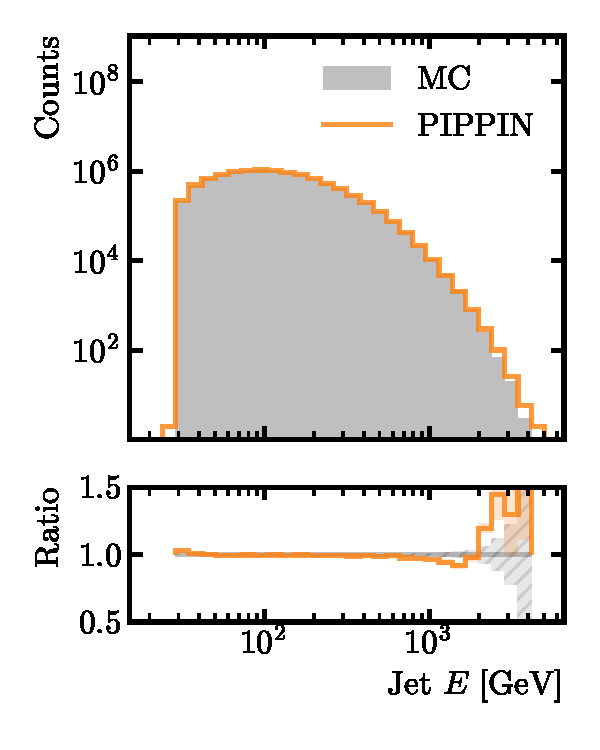
\includegraphics[width=0.32\textwidth]{Figures/jet_generation/pippin/marginals/marginal_jet_energy.pdf}
    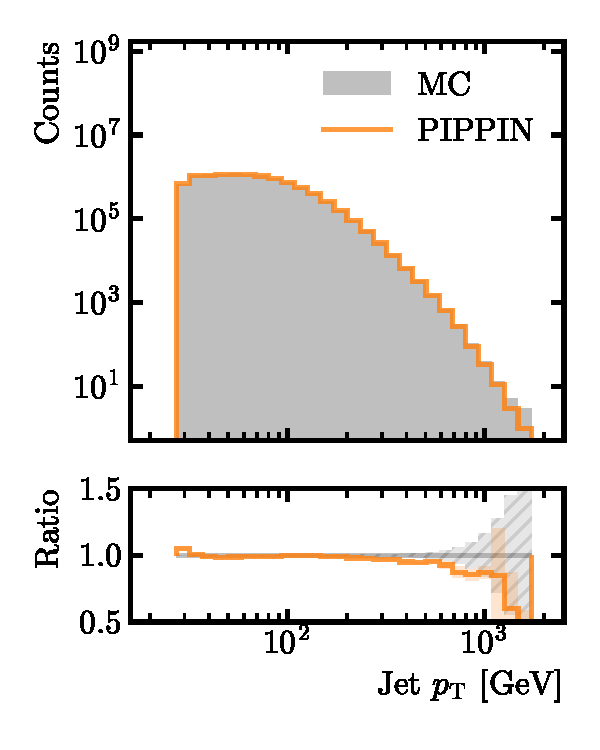
\includegraphics[width=0.32\textwidth]{Figures/jet_generation/pippin/marginals/marginal_jet_pt.pdf} \\
    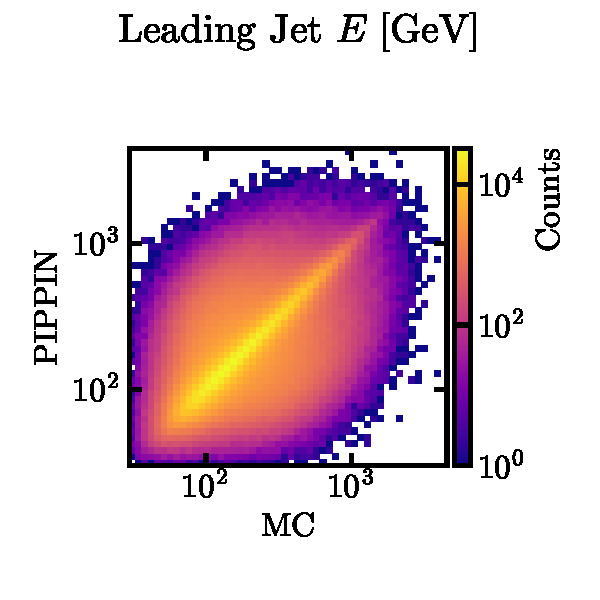
\includegraphics[clip, trim=0cm 0cm 0cm 2.5cm, width=0.32\textwidth]{Figures/jet_generation/pippin/marginals_2D/marginal2D_jet_energy.pdf}
    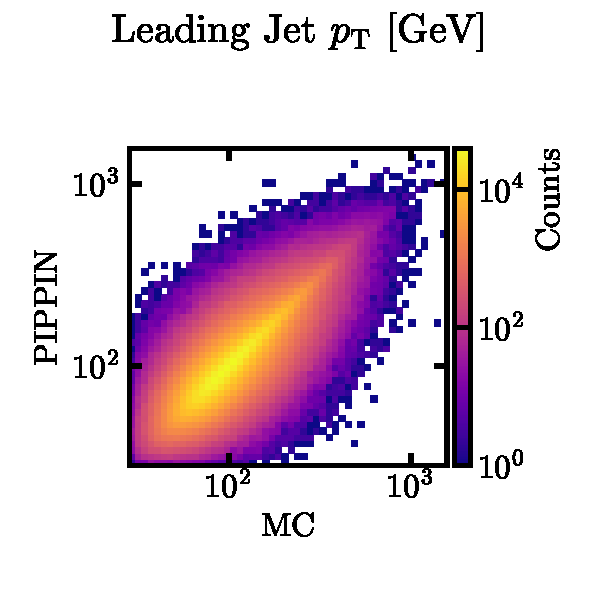
\includegraphics[clip, trim=0cm 0cm 0cm 2.5cm, width=0.32\textwidth]{Figures/jet_generation/pippin/marginals_2D/marginal2D_jet_pt.pdf}
    \caption{
        The marginal and conditional distributions of the predicted leading jet energy and \pt from the PIPPIN model compared to the full MC pipeline.
    }
    \label{fig:pippin_jet}
\end{figure}

\begin{figure}[htb]
    \centering
    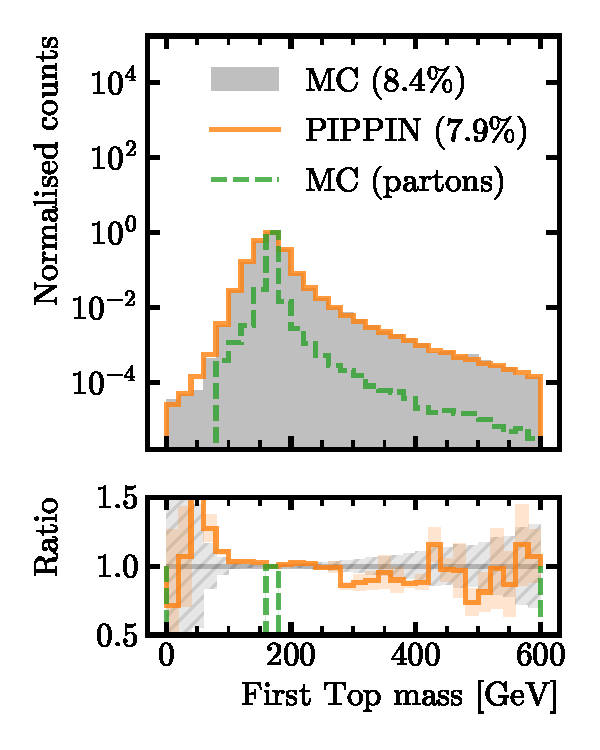
\includegraphics[width=0.32\textwidth]{Figures/jet_generation/pippin/masses/mass_top1.pdf}
    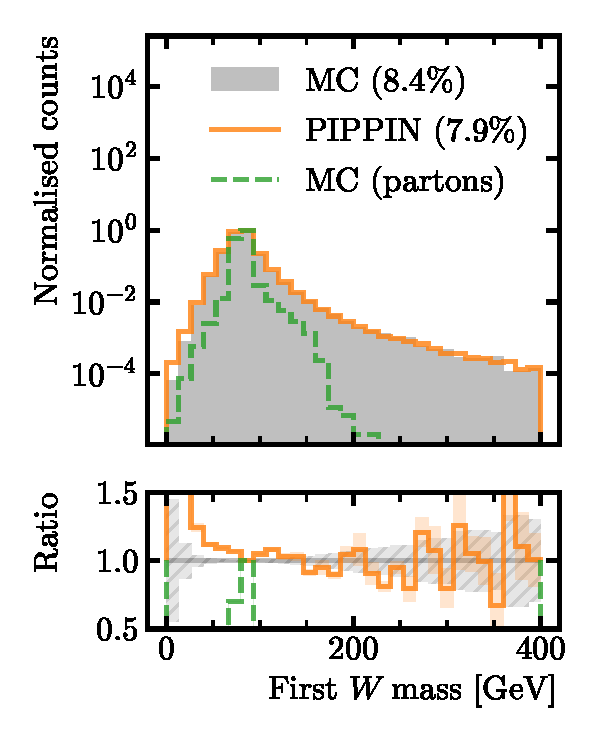
\includegraphics[width=0.32\textwidth]{Figures/jet_generation/pippin/masses/mass_w1.pdf}
    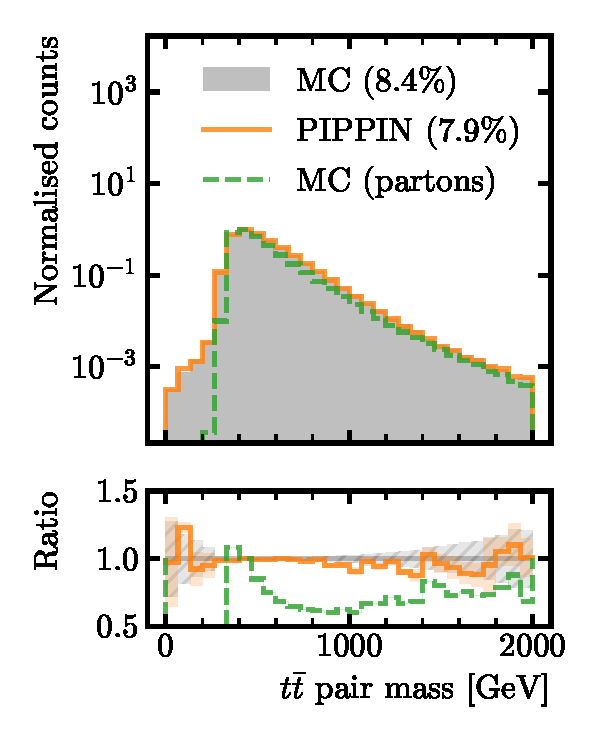
\includegraphics[width=0.32\textwidth]{Figures/jet_generation/pippin/masses/mass_ttbar.pdf}
    \caption{
        The marginal distributions of the reconstructed top quark, W boson, and \ttbar invariant masses from the PIPPIN model compared to the full MC pipeline.
        Also shown is the parton level mass.
        The percentages indicate the proportion of events for which all partons were unambiguously matched and therefore present in these plots.
    }
    \label{fig:pippin_mass}
\end{figure}

\begin{table}[htb]
    \centering
    \renewcommand{\arraystretch}{1.5}
    \caption{Comparison of the PIPPIN model with OTUS and Turbo-Sim on the full forward simulation task. Quoted values are the Kolmogorov-Smirnov distances between the model and the reco-level MC distributions.}
    \label{tab:pippin}
    \begin{tabular}{llllllll}
    \toprule
              & \multicolumn{3}{c}{Reco. objects} & \multicolumn{4}{c}{Underlying particles}                                                                           \\
    \cmidrule(l){2-4} \cmidrule(l){5-8}
    Model     & $p_y^{\text{jet}_1}$              & $p_z^{\text{jet}_1}$                     & $E^{\text{jet}_1}$ & $m^{t\bar{t}}$ & $m^{W_1}$ & $m^{t_1}$ & $m^{t_2}$ \\    \midrule
    OTUS      & 3.78                              & 2.39                                     & 5.75               & 15.8           & 11.7      & 14.1      & 24.9      \\
    Turbo-Sim & 2.89                              & 10.3                                     & 4.43               & 2.97           & 7.72      & 5.20      & 8.52      \\
    PIPPIN    & 0.07                              & 0.14                                     & 0.11               & 0.30           & 1.75      & 0.74      & 0.50      \\
    \bottomrule
\end{tabular}

\end{table}

\FloatBarrier

\section{Diffusion for Anomaly Detection}
\label{sec:drapes}

We developed the \pcdroid model to generate background templates for anomaly detection in jet structure.
This section is a brief summary of the work presented in~\textcite{Drapes}.

\subsection{CWoLa and Cathode}
\label{sec:cwolacathode}

As explained in \Cref{ch:sm}, there is reason to believe that the current understanding of physics is incomplete.
However, despite extensive analyses optimized for various BSM models, no significant evidence of new physics has been found.
Recently, broader anomaly detection methods have gained focus.
These searches are not highly sensitive to specific models but aim for a broader range of new physics scenarios.

A key technique in new physics searches is the bump hunt, which identifies localized data excesses, often expressed as a resonance in invariant mass.
Standard bump hunts are limited by the need to define a region in phase space enriched with enough BSM signal events to be statistically significant over the SM background.
Machine learning classifiers can provide a filter to reduce the amount of background present and thus enhance the power of the search.
However, training these models in a signal-agnostic way is challenging.

One such approach called CWoLa~\cite{cwola} trains a classifier to distinguish between data in the signal region (SR), which is assumed to be a mixture of signal and background events ($s+b$), versus some reference background ($b'$).
If the reference background $b'$ matches closely the true background $b$, then the ideal classifier that separates $s+b$ from $b'$ will also separate $s$ from $b$.

Constructing the reference background template now becomes the central challenge, and several methods have been proposed~\cite{cathode, salad, CURTAINs, feta, lacathode}.
One of the first methods, Cathode~\cite{cathode}, identifies the SR by a slice in some one-dimensional variable $c$, flanked by two sidebands.
Each data sample is defined by the slice variable $c$ and additional features $\x$.
A conditional generative model is trained using data from the sidebands to learn $p_\theta(\x|c_{\text{SB}})$, and the template is constructed by sampling from this model using $c$ values in SR, $x_{\text{SR}} \sim p_\theta(\x|c_{\text{SR}})$.
This method is highly effective, provided that the generative model can accurately capture the correlations between $c$ and $\x$, and can interpolate to unseen values of $c_\text{SR}$ during inference.
As long as the signal contamination in the sidebands is much lower than in the SR, the reference background can still lead to a good CWoLa classifier usable for enhanced bump hunts.

\drapes follows this approach, using a diffusion model as the generator.

\subsection{Experiments}

For this study, we used the LHCO R\&D Dataset~\cite{LHCO}, which has become a standard candle for performance in anomaly detection.
This is a di-jet dataset with a mixture of BSM and QCD events.
The slice variable is taken to be the di-jet mass, and the SR is defined as $m_{jj} \in [3.0, 3.7]~\TeV$.

We constructed two diffusion models for this task.
One which would generate purely the high-level features (\drapes HLV), where $\x$ is a one-dimensional vector, as this would allow us to compare the method to other models.
We used the same features as many of the existing models~\cite{CURTAINs, feta, lacathode}, including each jet's individual masses and subjettiness ratios.
The second model would generate the complete set of jet constituents, also called the low-level features (\drapes LLV).
Each jet is defined by a set of up to 150 constituents, similar to JetNet150.
The dijet event, therefore, has up to 300 individual particles.
We used the same setup for both models as \pcdroid but with a basic MLP instead of a transformer encoder for \drapes HLV.

The CWoLa classifier for \drapes HLV was a simple MLP with two hidden layers, while for \drapes LLV we used a three-layer transformer encoder.

As benchmarks, we compare to an over-idealised classifier, which uses actual background events as the template ($s+b$ vs $b$), and a supervised classifier trained with correct labels ($s$ vs $b$).
The primary performance metric is the significance improvement $SI$, defined as the number of signal events divided by the square root of the number of background events passing the CWoLA filter.

The classifier's performance trained on the \drapes HLV template is compared to the previous state-of-the-art model \FfF in \Cref{fig:drapes_hlv}.
For all levels of initial signal injection, \drapes provides a higher level of $SI$ than \FfF.
All methods, including the idealised classifier, drop off at around 500 injected signal events.
This is because we reach the CWoLa limit of the dataset, whereby the signal presence is too low for a $s+b$ vs $b$ classifier to learn to distinguish $s$ vs $b$.
\drapes performs better than the over-idealised classifier in some cases as we can increase the $b'$ statistics by an arbitrary amount, so we sample from the diffusion model until the performance saturates.
In contrast, the over-idealised classifier is limited to the number of QCD events in the dataset.

\begin{figure}[hbpt]
    \centering
    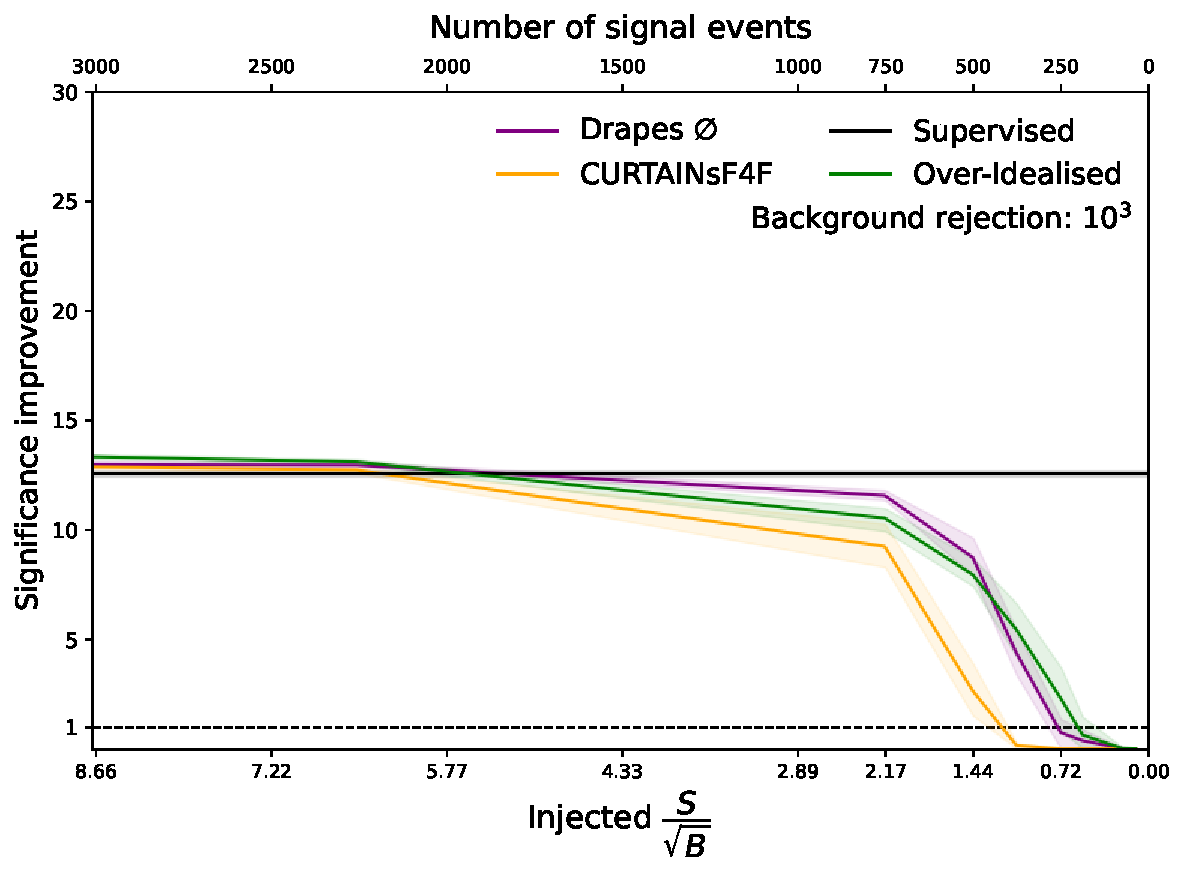
\includegraphics[width=0.49\textwidth]{Figures/jet_generation/drapes/og_compare_rej_1000_sic_vs_nsig.pdf}
    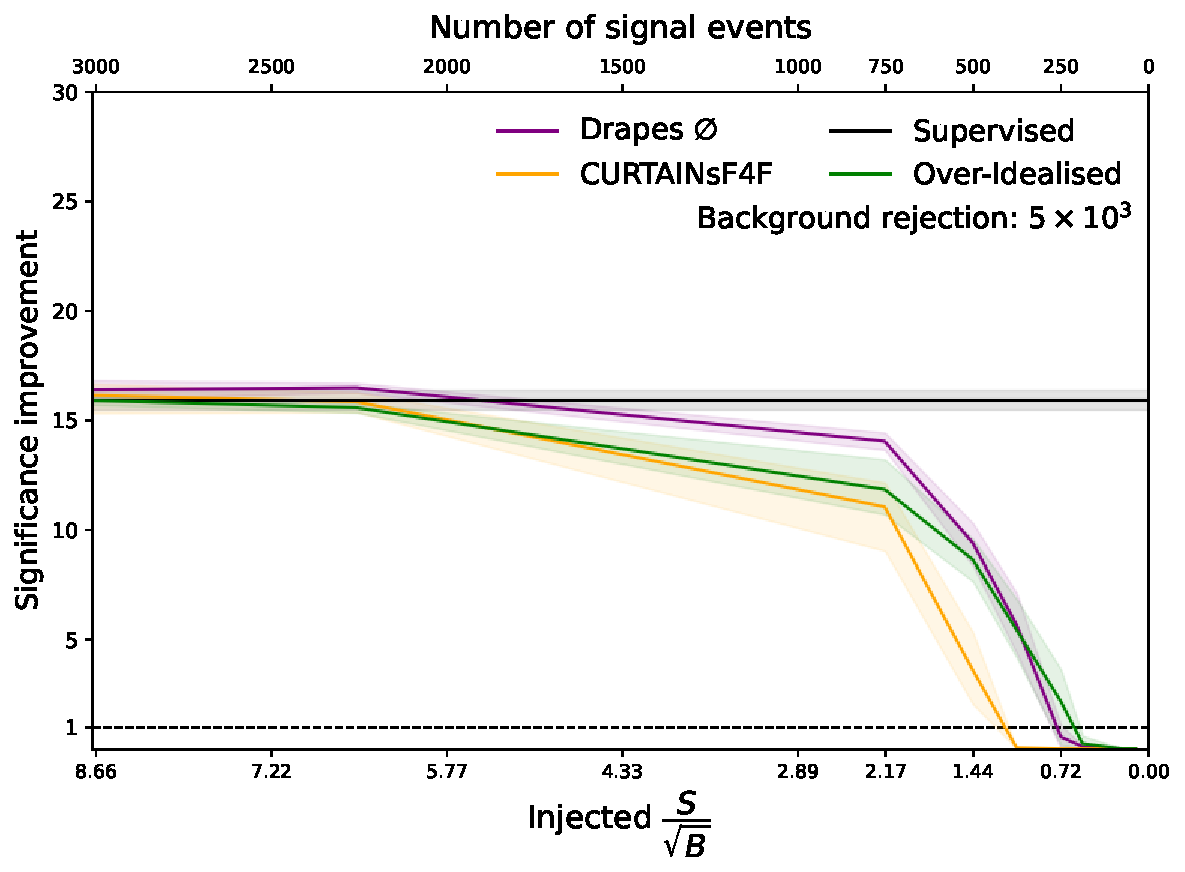
\includegraphics[width=0.49\textwidth]{Figures/jet_generation/drapes/og_compare_rej_5000_sic_vs_nsig.pdf}
    \caption{Significance improvement at fixed background rejection rates of $10^3$ (left) and \mbox{$5 \times 10^3$} (right) as a function of the number of signal events in the signal region, \mbox{$3300\leq m_{jj}<3700~\GeV$}, for \drapes, \FfF, Supervised, and Over-Idealised.
        The injected significance measured from the number of signal and background events in the signal region before applying a cut $\frac{S}{\sqrt{B}}$ is also shown.
        The lines show the mean value of fifty independent classifiers, with the shaded band representing a 68\% uncertainty.
    }
    \label{fig:drapes_hlv}
\end{figure}

The performance of \drapes~(LLV) with varying signal amounts is shown in \cref{fig:drapes_llv}.
The first thing to note is that when using the low-level features, the supervised benchmark yields an $SI=23.5$ at $r_b=1000$, much higher than the supervised benchmark using the high-level features, $SI=13.5$.
This increase in performance shows the potential sensitivity enhancements for searches operating on low-level features.
\drapes~LLV surpasses the high-level supervised model easily; however, to do so, it needs around 2000 signal events injected into the signal region, which corresponds to a significance already of 5.
In this setting, no extra anomaly detection methods would be needed, and this excess would easily be found by a simple bump hunt.
Unfortunately, the performance of \drapes~LLV drops off significantly below 2000 signal events and becomes worse than the high-level approach in the regions where we need it most.
This observation is consistent with a similar study contemporaneously to this work~\cite{FullPhaseSpace}.

A reason for this drop-off in performance is that CWoLa classifiers using neural networks lose sensitivity as input dimensionality increases, especially with signal-insensitive inputs~\cite{lacathode}.
This effect is heightened as the number of signal events decreases.
Many methods are reverting to decision trees as they seem better suited for CWoLa style training~\cite{TreebasedAlgorithmsWeakly, AnomalyDetectionPresence}.
Moving from a few high-level variables to jet constituents multiplies the input dimensionality by over 150, severely affecting weakly supervised neural networks.
The so-called CWoLa limit, the minimum number of required signal events injected into the dataset, was increased when moving to this higher dimensional regime.
Therefore, this loss in sensitivity is due to the CWoLa approach, and more work needs to be done to find a way to train larger models on point cloud data in a weakly supervised way.

\begin{figure}[hbpt]
    \centering
    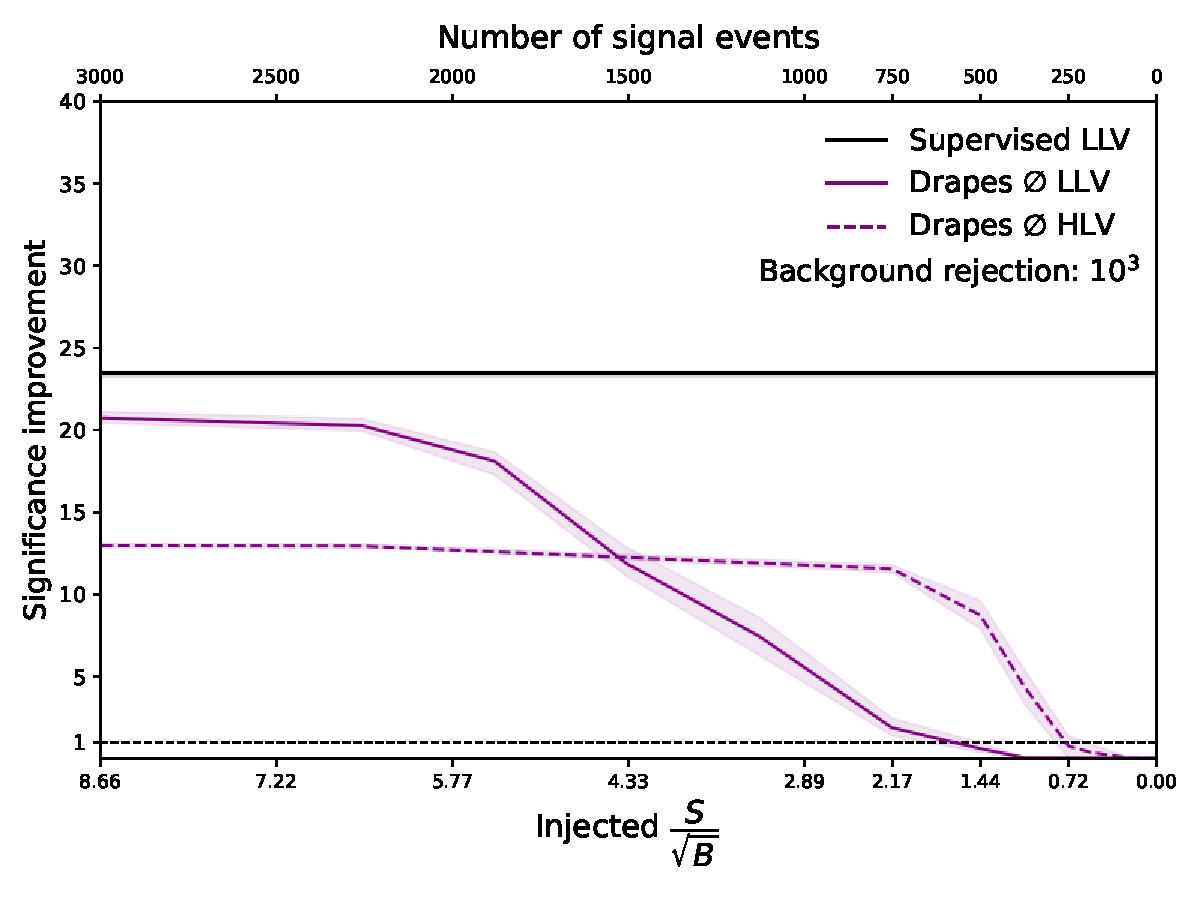
\includegraphics[width=0.49\textwidth]{Figures/jet_generation/drapes/lowlevel_null_sic_vs_soverb_rej_1000.pdf}
    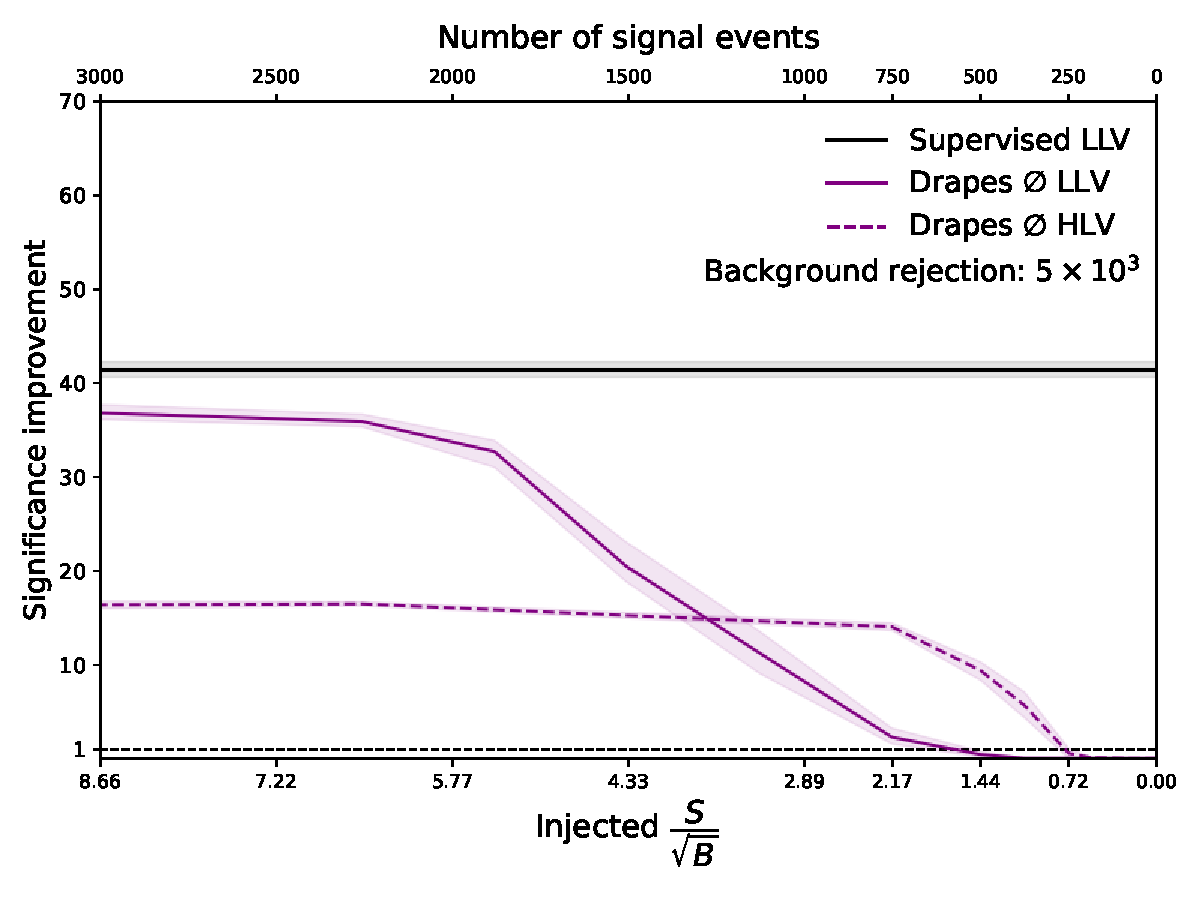
\includegraphics[width=0.49\textwidth]{Figures/jet_generation/drapes/lowlevel_null_sic_vs_soverb_rej_5000.pdf}
    \caption{Significance improvement at fixed background rejection rates of $10^3$ (left) and \mbox{$5 \times 10^3$} (right) as a function of the number of signal events in the signal region, \mbox{$3300\leq m_{jj}<3700~\GeV$}, for \drapes using low level jet constituents (LLV) or high level variables (HLV). The injected significance measured from the number of signal and background events in the signal region before applying a cut $(\frac{S}{\sqrt{B}})$ is also shown. The lines show the mean value of fifty independent classifiers, with the shaded band representing a 68\% uncertainty. The supervised classifier is trained on low level jet constituents is shown for reference.}
    \label{fig:drapes_llv}
\end{figure}

\subsection{Conclusion}

We have demonstrated that diffusion models can generate templates for CWoLa classifiers in anomaly detection.
The \drapes model generated templates led to increased sensitivity in CWoLa style signal searches, outperforming the previous state-of-the-art model \FfF.
However, when transitioning to the full jet constituent space, we found a significant drop in sensitivity when the injected signal significance was below 4.33.
Due to corroborating studies, we believe this is due to the failure of a large transformer being trained with highly noisy labels rather than issues with the template generation.
